\documentclass[a4paper, 11pt]{article}

\usepackage[utf8]{inputenc}
\usepackage[top=2.5cm, left=2.5cm, right=2.5cm, bottom=3.2cm]{geometry}

% Load trebuchet in for the title and section fonts
\usepackage{fontspec}
\newfontfamily\titlefont{Trebuchet MS}
\setmainfont{XITS}

\usepackage[fleqn]{amsmath}
\usepackage[mathrm=sym]{unicode-math}
\setmathfont{XITS Math}

% Word spacing and formatting
\usepackage[british]{babel}
\usepackage{csquotes}
\usepackage{microtype}
%\usepackage[none]{hyphenat} % prevent hyphenation to allow easy copy and paste to word template later


\usepackage{xcolor}
\usepackage{mdframed}

% Section header styling
\usepackage{sectsty}
\sectionfont{\titlefont\Large\raggedright}
\subsectionfont{\titlefont\large\raggedright}
\subsubsectionfont{\it\titlefont\normalsize\raggedright}

% Set up caption styling
\usepackage{caption}
\DeclareCaptionFormat{capfont}{\titlefont\small#1#2#3}
\captionsetup{format=capfont,font=bf,labelsep=period} 

% Hyperlinks
\usepackage[colorlinks=true, allcolors=blue]{hyperref}
\urlstyle{same}


\usepackage[detect-all]{siunitx} % SI Unit package

%\renewcommand{\labelitemi}{}
\renewcommand{\labelitemii}{$\circ$}
\renewcommand{\labelitemiii}{\footnotesize$\blacksquare$}

% Citations
\usepackage[
    backend=biber,
    bibencoding=utf8,
    sorting=nyt,
    style=apa,
    url=false, % include url in reference
    doi=false, % include doi in reference
    %sorting=none, % sorting of citations
    % autocite=superscript, % autocite becomes superscript
    maxcitenames=2, % Max names displayed when citing in text
    %maxbibnames=20, % Max number of names disaplayed in the bibliography
    giveninits=true, % Use initials
    uniquename=init
]{biblatex}
%\setlength\bibitemsep{0.1\itemsep}
\renewcommand*{\bibfont}{\small}
\addbibresource{citations.bib}

% cross-referencing
\usepackage[noabbrev, capitalise]{cleveref}

\usepackage{wrapfig}
\usepackage[]{graphicx}
\usepackage{standalone}
\usepackage{subfig}
\usepackage{tikz}
\usepackage{tikz-3dplot}

\usepackage{booktabs}
% https://tex.stackexchange.com/questions/12703/how-to-create-fixed-width-table-columns-with-text-raggedright-centered-raggedlef
\usepackage{array}
\newcolumntype{L}[1]{>{\raggedright\let\newline\\\arraybackslash\hspace{0pt}}m{#1}}
\newcolumntype{C}[1]{>{\centering\let\newline\\\arraybackslash\hspace{0pt}}m{#1}}
\newcolumntype{R}[1]{>{\raggedleft\let\newline\\\arraybackslash\hspace{0pt}}m{#1}}


\begin{document}

{
  \titlefont
  \small
  \begin{wrapfigure}{r}{0.2\textwidth}
    \raggedleft
    \vspace{-0.2cm}
    
\includegraphics[width=1.8cm]{figs/design-logo.png}
  \end{wrapfigure}
  \noindent \textbf{INTERNATIONAL DESIGN CONFERENCE - DESIGN 2020}\\
  \url{https://doi.org/10.1017/dsd.2020.93}

  \vspace{2cm}

  \Large\noindent\textbf{DEMOCRATISING DESIGN THROUGH SURROGATE MODEL NEURAL NETWORKS OF COMPUTER AIDED DESIGN REPOSITORIES}

  \vspace{1cm}

  \normalsize \noindent J.\ Gopsill and S.\ Jennings \\[0.2cm]
  \footnotesize \noindent University of Bath, United Kingdom \\[0.1cm]
  \footnotesize \noindent J.A.Gopsill@bath.ac.uk\\

  \begin{mdframed}[backgroundcolor=gray!20] 
    \normalsize \noindent \textbf{Abstract} \\
    \normalfont The capability to manufacture at home is continually increasing with technologies, such as 3D printing. 
    However, the ability to design products suitable for manufacture and use remains a highly-skilled and knowledge intensive activity.
    This has led to `content creators' providing vast repositories of manufacturable products for society, however challenges remain in the search \& retrieval of models.
    This paper presents the surrogate model convolutional neural networks approach to search and retrieve CAD models by mapping them directly to their real-world photographed counterparts.
  \end{mdframed}

  \small \noindent \textit{Keywords: 3D printing, computer-aided design (CAD), design informatics, surrogate models,\\ convolutional neural networks}

  \vspace{0cm}
}


\section{Introduction}

3D printing has been recognised by many as the technology that will lead to the ``prosumption'' society where individuals are both producers and consumers of goods and services \parencite{hermans2015}. While 3D printing has democratised the manufacture of components due to its low-price and suitability for home use, many individuals in society are still limited in applying this technology due to the underlying Design \& Manufacture (D\&M) knowledge required to produce the Computer Aided Design (CAD) models required for the process.

To overcome this, a range of online CAD repositories have arisen where experts are able to upload their manufacturable models for others to download and print. These individuals are often referred to as ``content creators''. For example, Thingiverse holds 1,655,150 CAD models and sees millions of downloads every month\footnote{\url{https://www.thingiverse.com/about/}}, whilst GrabCAD features 4,030,000 produced by 6,920,000 content creators\footnote{\url{https://grabcad.com/library}}.
These CAD data lakes have since become an emergent area for research with researchers investigating the open source nature of design and ability to share knowledge, as well as the barriers in the application of stored 3D models due to the variety in geometric representations used (e.g. .stl, .ipt, .iges, .f3d) \parencite{buehler2015,baumann2018,alcock2016}.
Given the wealth of available models for individuals to download, the challenge that this paper identifies lies in search and retrieval.

Search \& retrieval is currently achieved by individuals having the necessary knowledge and understanding to describe the models they have created as well as consumers in the search terms used. Descriptions that should embody both form and application of the model. This is where one encounters all the traditional challenges of text-based search and retrieval. Given the model geometry, could one not use this to support the search and retrieval of models and further democratise the D\&M process for 3D printing?

This paper answers this question by applying Convolutional Neural Networks (CNNs) trained on a surrogate model of rendered images produced from CAD files in online repositories. A surrogate model in this context is a training set that has been generated to simulate the real-world data that will be provided to the CNN for prediction. Training through a surrogate model mitigates one of the biggest challenges in CNNs, which is having a rich labelled dataset to train on. The trained CNN then allows individuals to take images/live video of real-world objects and have the CNN suggest the closest matching CAD model available in the repository, thereby meeting our overall objective of democratising 3D printing.

The related work in re-engineering CAD models is now discussed (\cref{sec:rel}). This is then followed by the description of the surrogate model Convolutional Neural Network and subsequent study used to evaluate the potential of the approach (\cref{sec:study}).
The results are then presented (\cref{sec:res}) followed by a discussion on future work (\cref{sec:dis}). The paper then concludes by highlighting the key findings from the study (\cref{sec:con}).

\section{Related work}\label{sec:rel}

Research into the generation of CAD models from real-world models can be grouped as single-image object recognition, multi-image to 3D object reproduction and object-scanning to 3D model reproduction. In addition, there have been a few studies showing the potential of Neural Networks for 3D geometry primarily focused on the matching of digital 3D geometry \parencite{zaki2016,maturana2015}. These are now discussed in relation to their potential for democratising the D\&M process of 3D printing.

\subsection{Single-image object recognition}

Single-image object reproduction estimates 3D geometry from 2D images. When recovering polyhedral objects, reconstruction algorithms assume parallel projection from an oblique view - a valid assumption for relatively short objects where perspective projection is negligible \parencite{lee2011}.

Using ``large differences between neighbouring elements by sharp spatial gradient'', boundary detection identifies object edges \parencite{liu2005}. 
These edges are built into a surface using rectification to remove objective distortion and image vanishing points to produce affine geometry.
Affine geometry is converted to a parallel original-image projection using circular vanishing points. A control polyhedron is applied to the surface, followed by control-point cubic corner inflation to produce 3D representations \parencite{jha2014}.

Single-image object reproduction is only capable of reproducing visible views, meaning the final model inevitably lacks detail, unless it is rotationally symmetric with the view used (\cref{fig:1a}) \parencite{van19983d}. 
Single images lose true depth information of a scene point in 2D projection, meaning depth recovery is required to re-produce a 3D object \parencite{liu2005}. 
Hence single-image object recognition is limited to (and only advantageous in) simple geometry cases such as a logo, where one view can capture the entire geometry.

\begin{figure}[t!]

    \hfill{}
    \subfloat[Single-image~\cite{van19983d}]{
        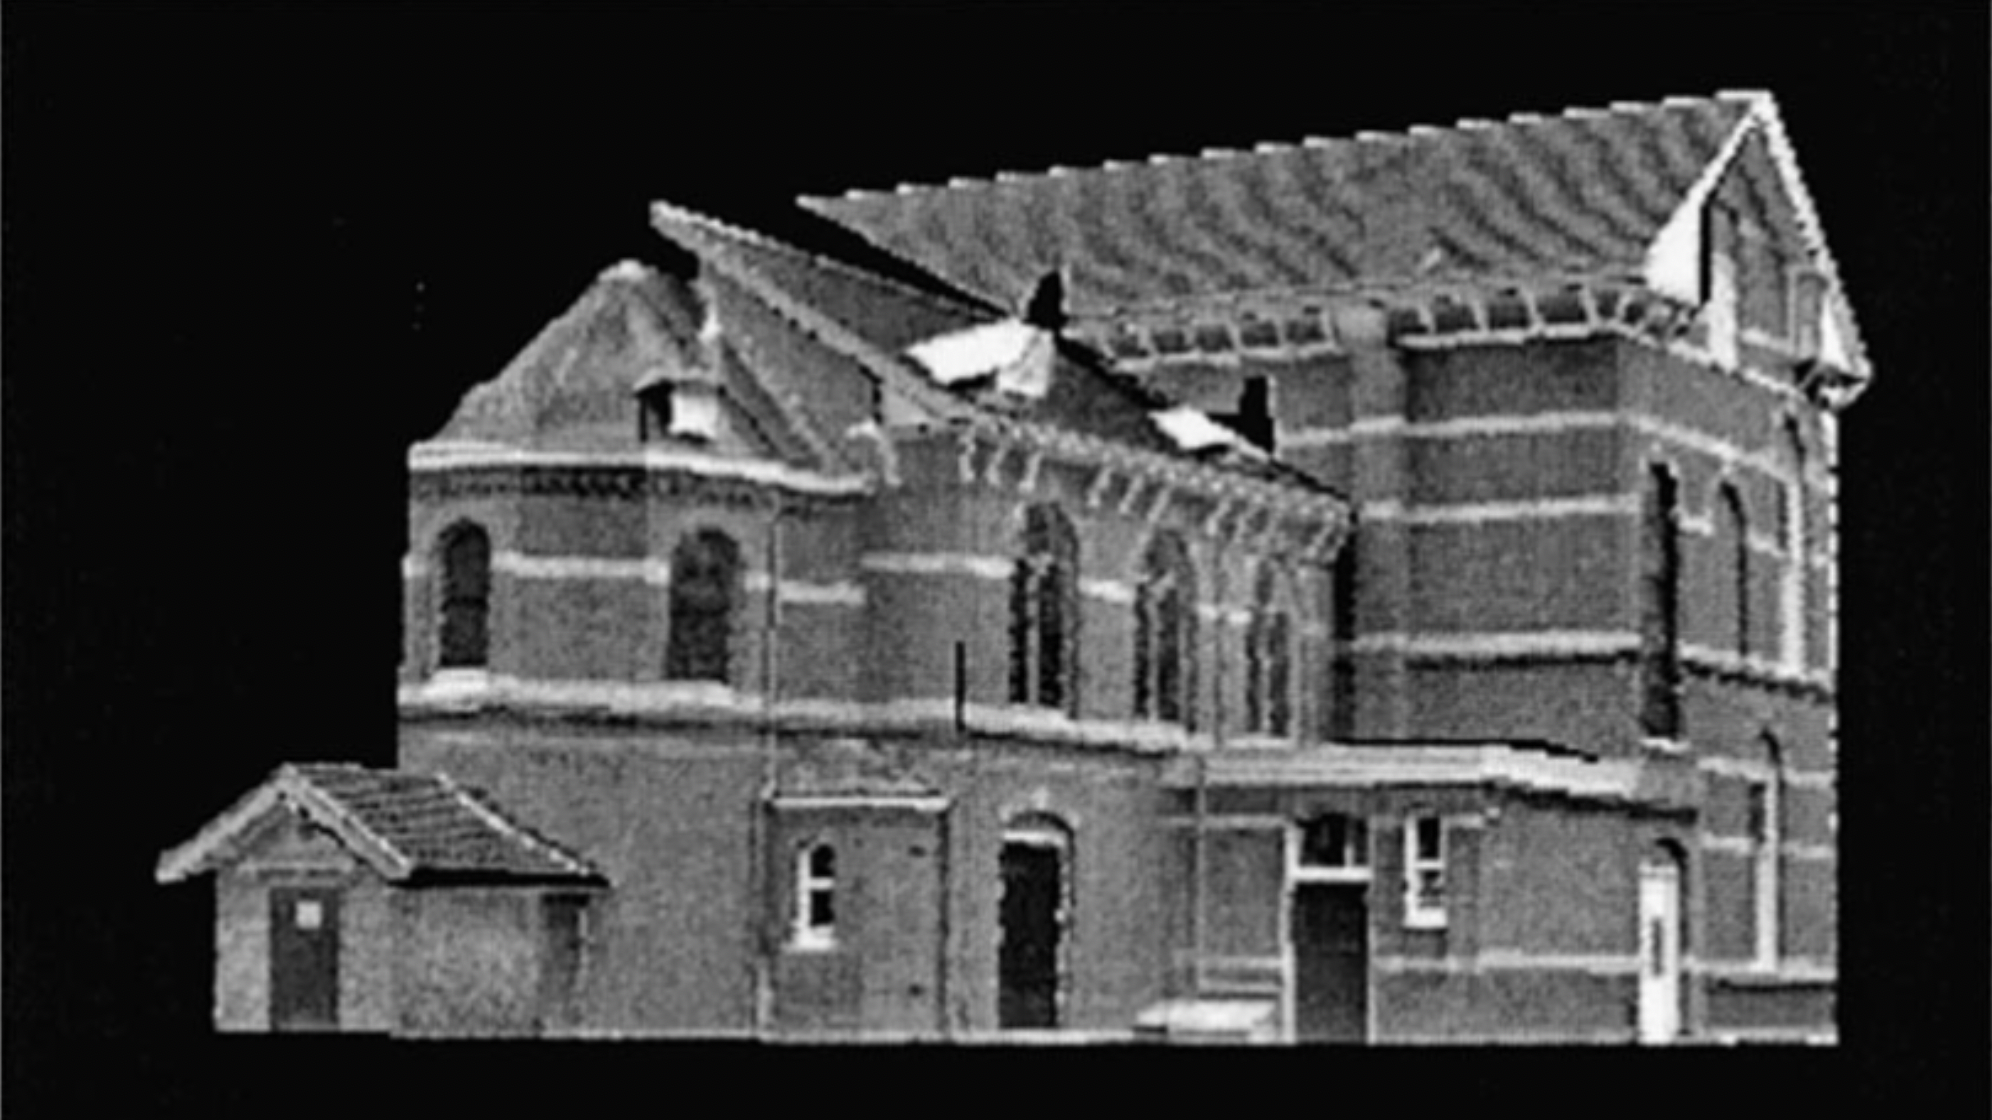
\includegraphics[height=3cm]{figs/single-image.png}
        \label{fig:1a}
    }
    \hfill{}
    \subfloat[Multi-image~\cite{arc2019}]{
        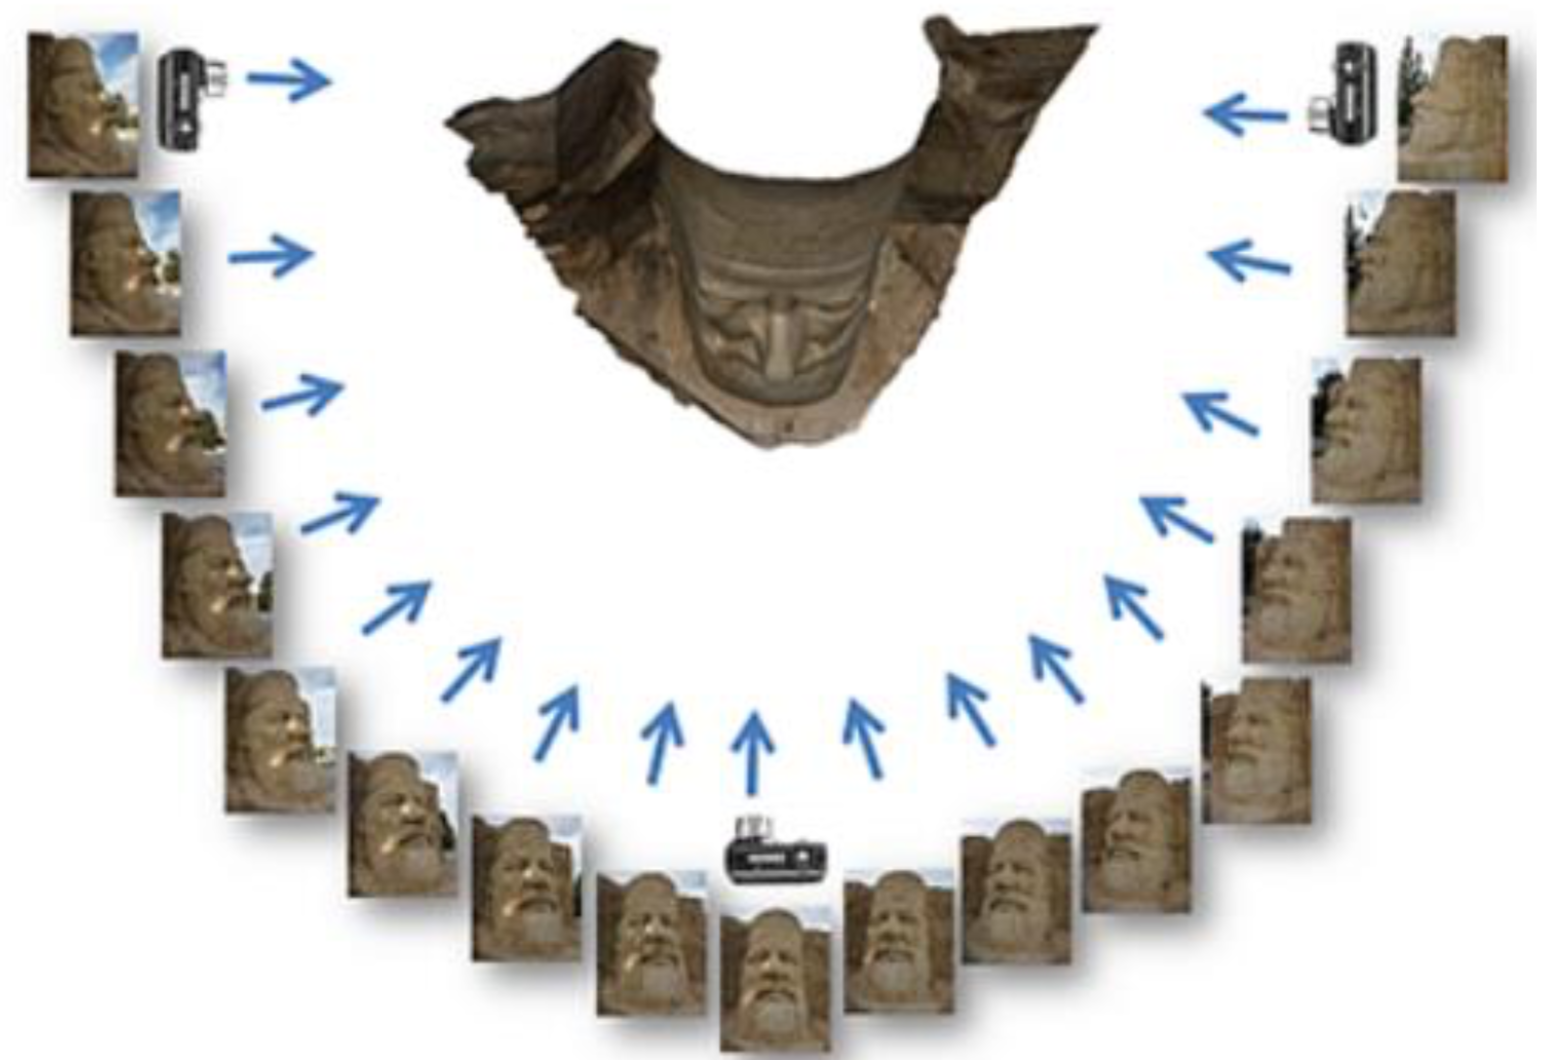
\includegraphics[height=3cm]{figs/multi-image.png}
        \label{fig:1b}
    } 
    \hfill{} 
    
    \leavevmode \\
    
    \hfill{}
    \subfloat[Makerbot digitiser]{
        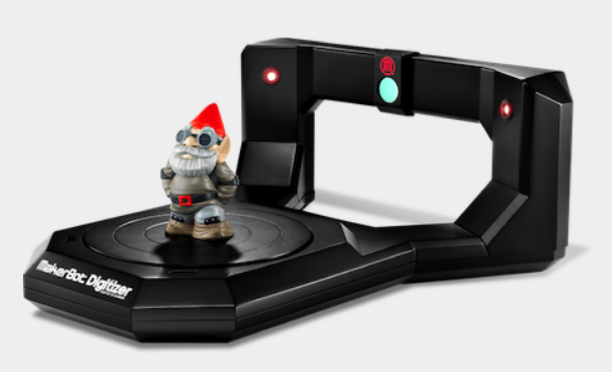
\includegraphics[height=3cm]{figs/digitiser.png}
        \label{fig:1c}
    }
    \hfill{}
    \subfloat[CNN CAD-to-CAD matching~\cite{zaki2016}]{
        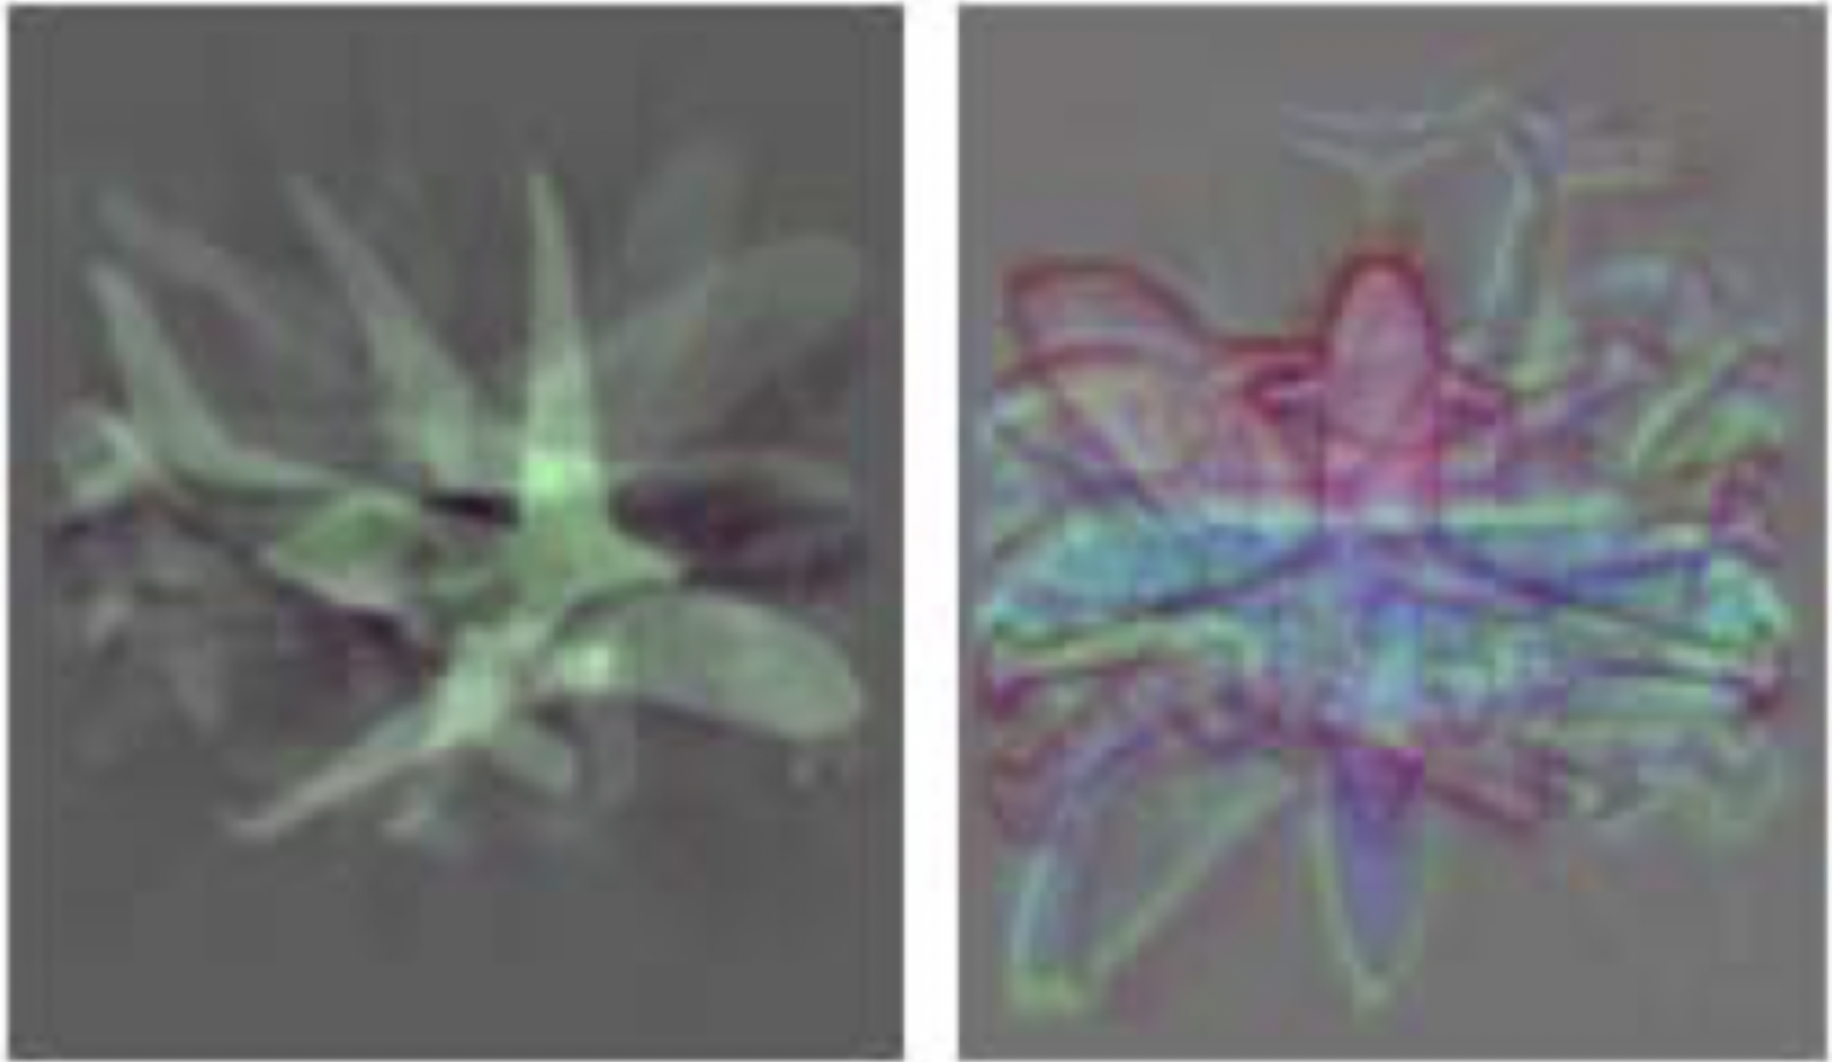
\includegraphics[height=3cm]{figs/cnn.png}
        \label{fig:1d}
    }
    \hfill{}
    
    \caption{Approaches to 3D model reproduction}
    \label{fig:1}
\end{figure}

\subsection{Multi-image to 3D object reproduction}

Multi-image to 3D object reproduction uses several object viewpoints to build a 3D model (\cref{fig:1b}), known as multi-view stereopsis \parencite{furukawa2009}. Multi-view stereopsis uses a reconstruction pipeline to produce 3D object surfaces. Camera parameters, such as focal length, are estimated by comparing images, allowing image calibration. Common features are identified and matched between images, producing connection points. An initial view is selected, and additional views added sequentially through connecting points, producing a sparse cloud representation of the object. The sparse-point cloud is converted into a dense-cloud by computing image pixel depths across surfaces of corresponding object images. This produces a depth-map, filtered and converted to a detailed 3D object model \parencite{tingdahl2011}.

ARC3D is a commercial tool that applies this technique for 3D geometry generation (Figure 1b). The tool is advantageous as the scanned object size is scale free enabling both small and large items to be re-created. However, the tool can find ‘weak’ textures, such as skin and reflective surfaces, challenging with the resulting surface often requiring post-processing tools to produce acceptable surface resolution \parencite{arc2019}.
In addition, the method re-constructs a surface and further checks are required to ensure the surface forms a body and that the resulting body is suitable of 3D printing.
This post-processing requires knowledge, skills and tools in digital image processing and surface geometry manipulation, meaning poor usability for the home consumer.

\subsection{Object-scanning to 3D model reproduction}

Another approach that has been taken is to apply object scanning of the model using distance measuring devices, such as lasers. These systems create a point-cloud, which is used to create a mesh of the object. Filtering techniques, such as Kalman filters, reduce surface noise and roughness effects of measurement uncertainty \parencite{weiss2009}.
The MakerBot Digitiser is one such example of a commercial solution that applies this approach (\cref{fig:1c}).

Challenges in this approach are in the time it takes to complete a scan (typically 12 min for the MakerBot Digitiser) and missing occluded surfaces often resulting in a convex hull of the item being scanned.
Post-scan, individuals are still required to the check the mesh to ensure it form a complete body.
Again, there is an underlying requirement for the individual to have knowledge of manipulating geometry.

\subsection{Convolutional neural networks}

Convolutional Neural Networks (CNN) have also been applied with the focus on matching digital 3D geometries. For example, \textcite{zaki2016} has trained a CNN on multi-view renders of 3D geometry and used these to cluster and classify other 3D geometries (\cref{fig:1d}).
A potential use case for this is the matching of similar parts across product families with a view to reduce the part variety in an organisations supply chain. 
While \textcite{maturana2015} have sought to augment depth mapped images with Neural Networks to develop voxel-based approximations of objects within a scene.

\subsection{Summary}

These results show the promise of CNNs as a means of supporting geometry matching and classification and this paper further contributes to this space by investigating the potential of CAD renders to form a surrogate model for the CNN to be trained on and its subsequent accuracy in classifying a set of real-world photographs. Achieving this would eliminate the need to build labelled datasets of real-world images featuring the objects of interest as well as being able to relate real-world objects to 3D printable CAD files. \cref{tbl:comparison} summarises the advantages and disadvantages of the four approaches.

The paper now continues into the development of the study to investigate the potential of surrogate model convolutional neural networks to democratise D\&M through the matching of 3D printable CAD files to real-world objects.

\begin{table}
  \caption{Comparing approaches to object reconstruction}
  \label{tbl:comparison}\footnotesize
  \begin{tabular}{L{0.3\textwidth} L{0.3\textwidth} L{0.3\textwidth}}
    \toprule
      Method & Advantages & Disadvantages \\
    \midrule
      Single-image object reproduction & 1. Computationally inexpensive. & 1. Applicable to 2D geometry with little to no 3D variation. \\
      & 2. Repeatable and explainable. & \\
      \midrule
  
      Multi-image to 3D object reproduction & 1. No limitation to object size. & 1. Generally, produces poor resolution surfaces \\
      & 2. Professional programs can produce reasonable resolution models. & 2. Post-processing software is required for optimal resolution. \\
      & & 3. Considerable digital toolchain and skillset required by the user. \\
  
      \midrule
      Object Scanning to 3D Image Reproduction & 1. Simple camera calibration & 1. Higher cost in comparison to other techniques. \\
      & 2. High resolution surfaces. & 2. Limited by types of surface that can be scanned. \\
      & 3. Dimensionally accurate models & 3. Long scanning time \\
  
      \midrule
      Convolutional Neural Networks & 1. Fast response in determining a match. & 1. Requires dataset to train on. \\
      & 2. New data can be added to the training. & 2. Requires considerable computational power to train. \\
      & 3. Returns CAD models & 3. Can return no matches. \\
    \bottomrule
  \end{tabular}
\end{table}



\section{Study}\label{sec:study}

The investigation into the potential of generating a surrogate model from CAD renders to train a CNN that will be used to evaluate real-world photos followed a four-step process.

\begin{enumerate}
  \item Model selection
  \item Generating the surrogate model
  \item Train
  \item Test \& refine
\end{enumerate}

The first step involved selecting a subset of CAD models held within GrabCAD that will be used to generate the surrogate model. With the models chosen, the surrogate model was developed. The process then preceded into training a series of CNNs using the surrogate model. To test the CNNs, a set of test images generated from real-world 3D printed versions of the CAD models was created and metrics on the accuracy of prediction were created. Following the results from the initial test, experiments were then performed to see how one could refine the model by reducing the computational cost of generating the surrogate model by reducing the number of images rendered and applying rotation, reflection and scaling augmentation strategies. Each step is now discussed in further detail.

\subsection{Model selection}

The parts selected are shown in \cref{fig:cad-models}. The rationale for their selection is that they were some of the most popular models on GrabCAD and feature a mixture of everyday objects individuals might wish to produce. In addition, models were selected based on having similar geometric profiles to test the level at which the CNN could differentiate between models. The primary example for this test is between the car and mouse (\cref{fig:car,fig:mouse}).

\begin{figure}[t!]
    
    \hfill{}
    \subfloat[Coffee Cup \parencite{borque2018}]{
        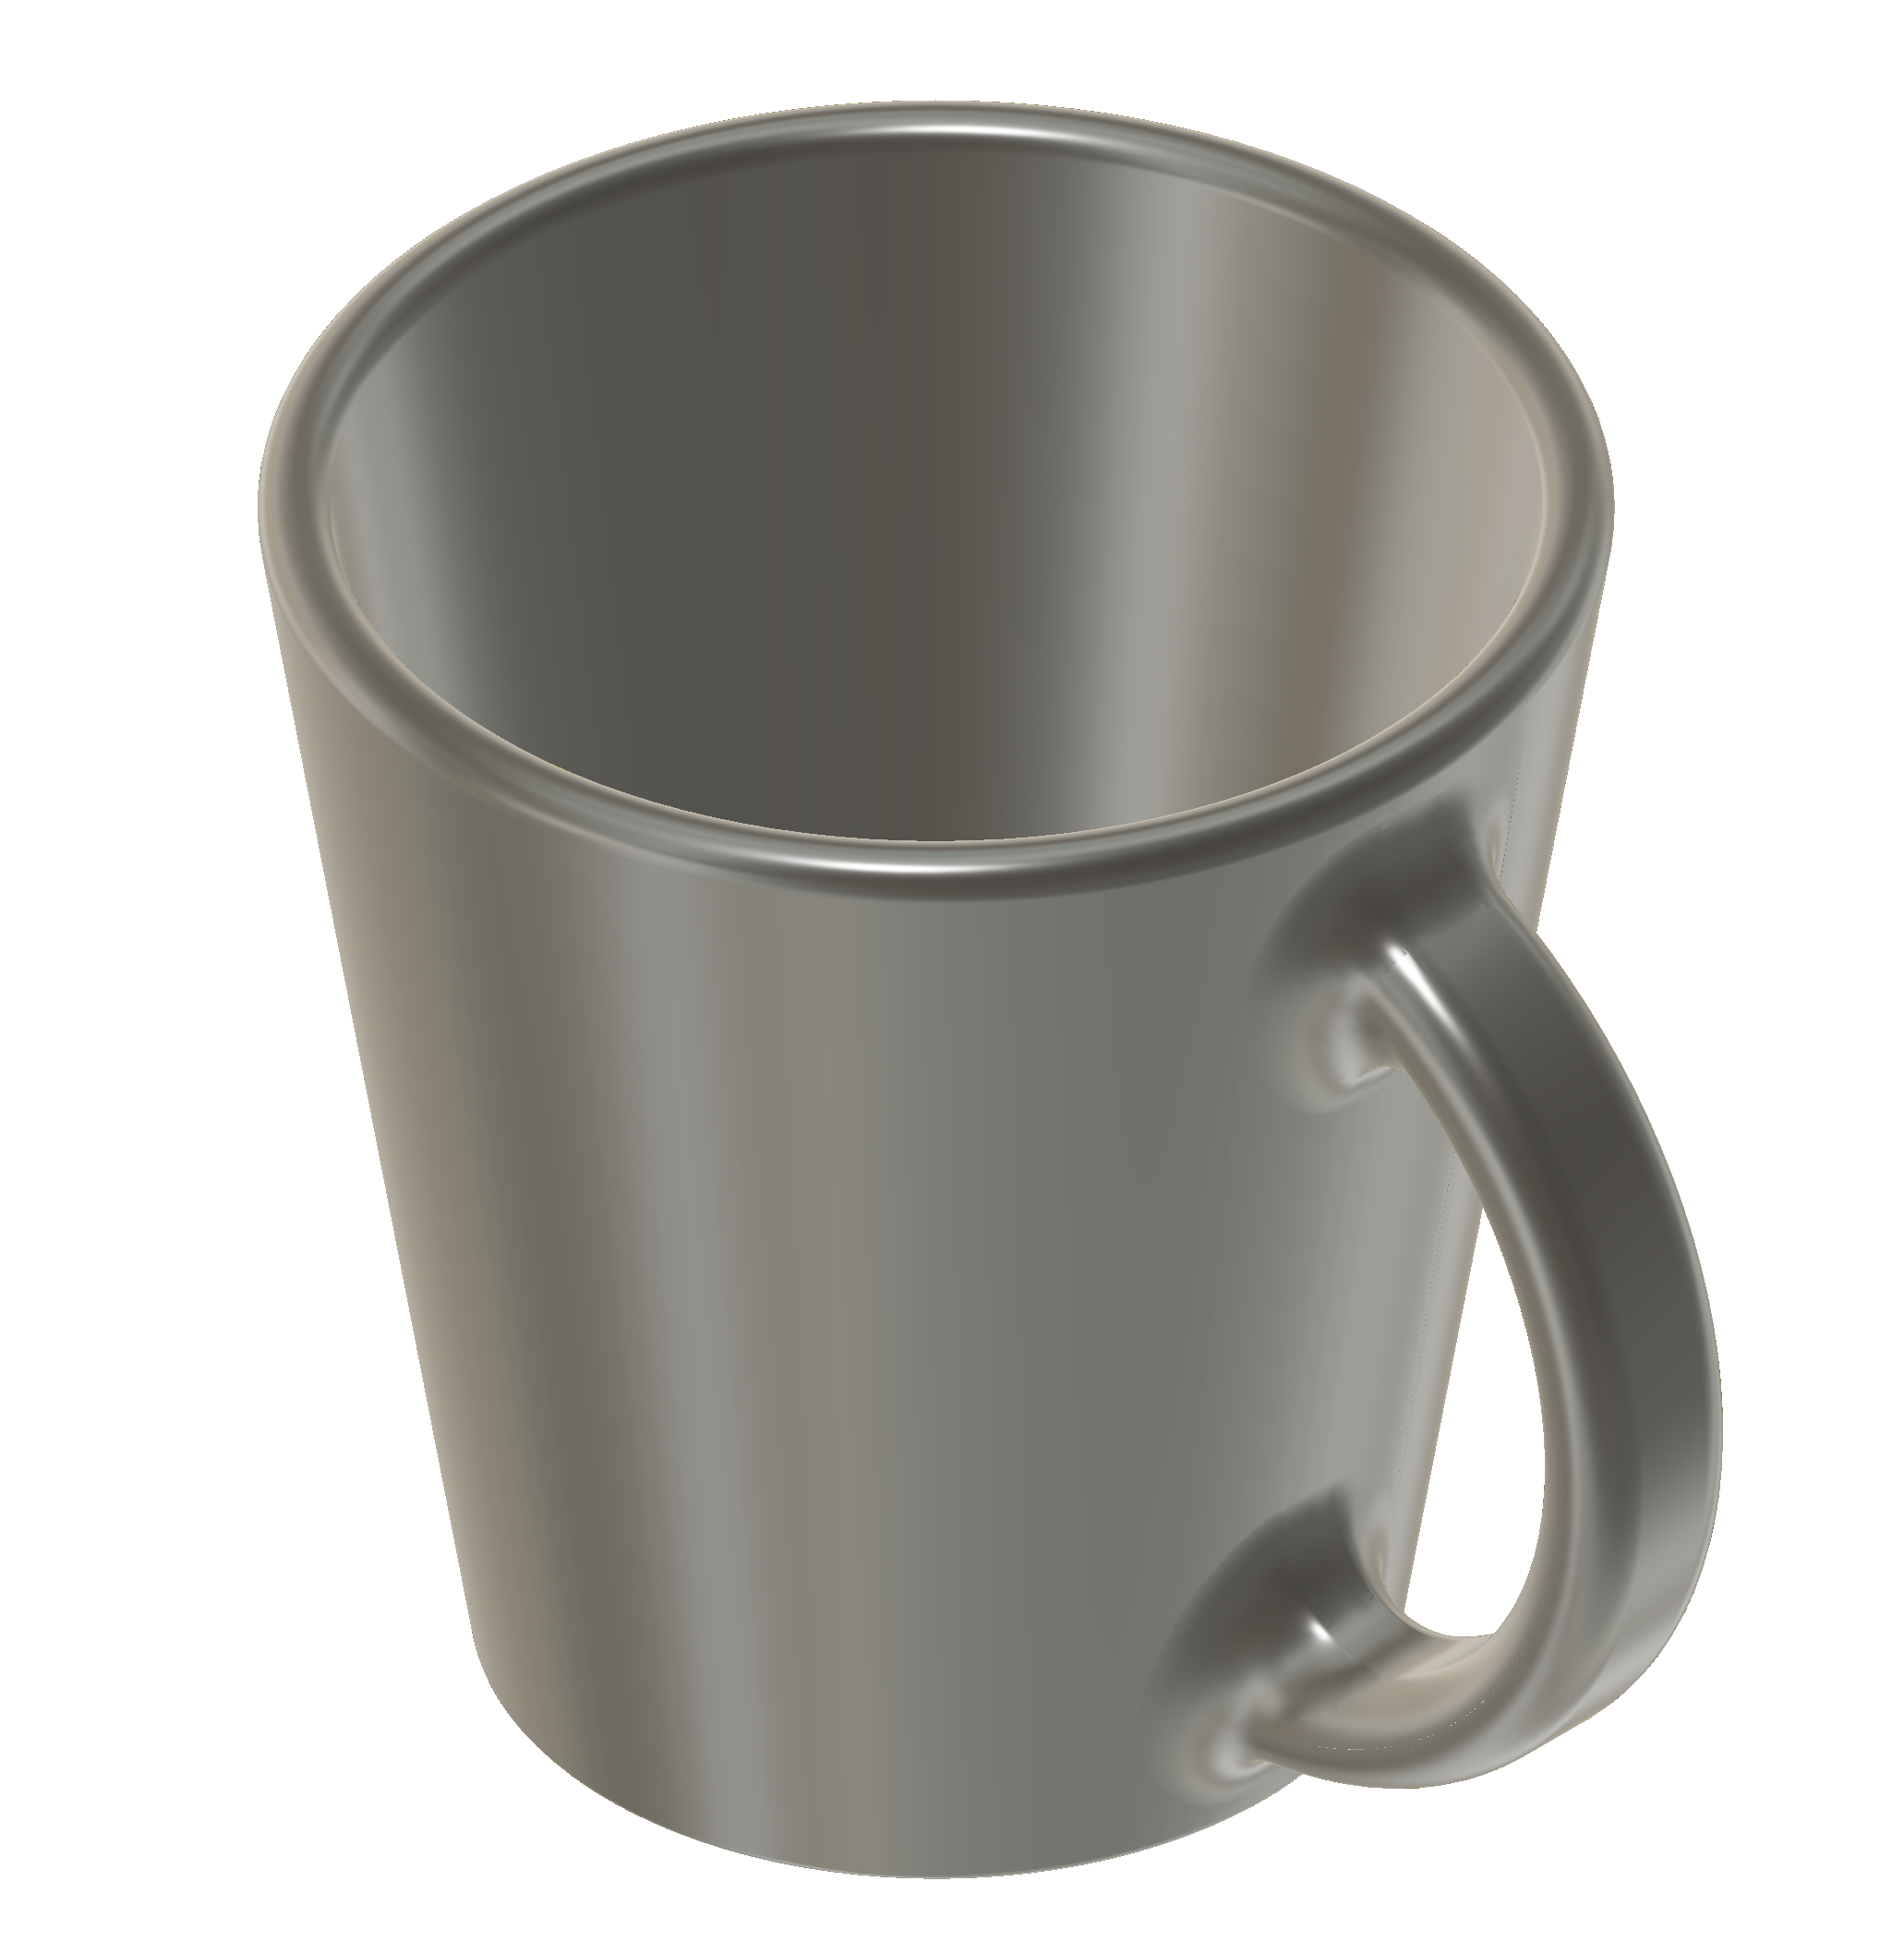
\includegraphics[height=2.8cm]{figs/cup.png}
    }
    \hfill{}
    \subfloat[Turbine \parencite{solanki2019}]{
        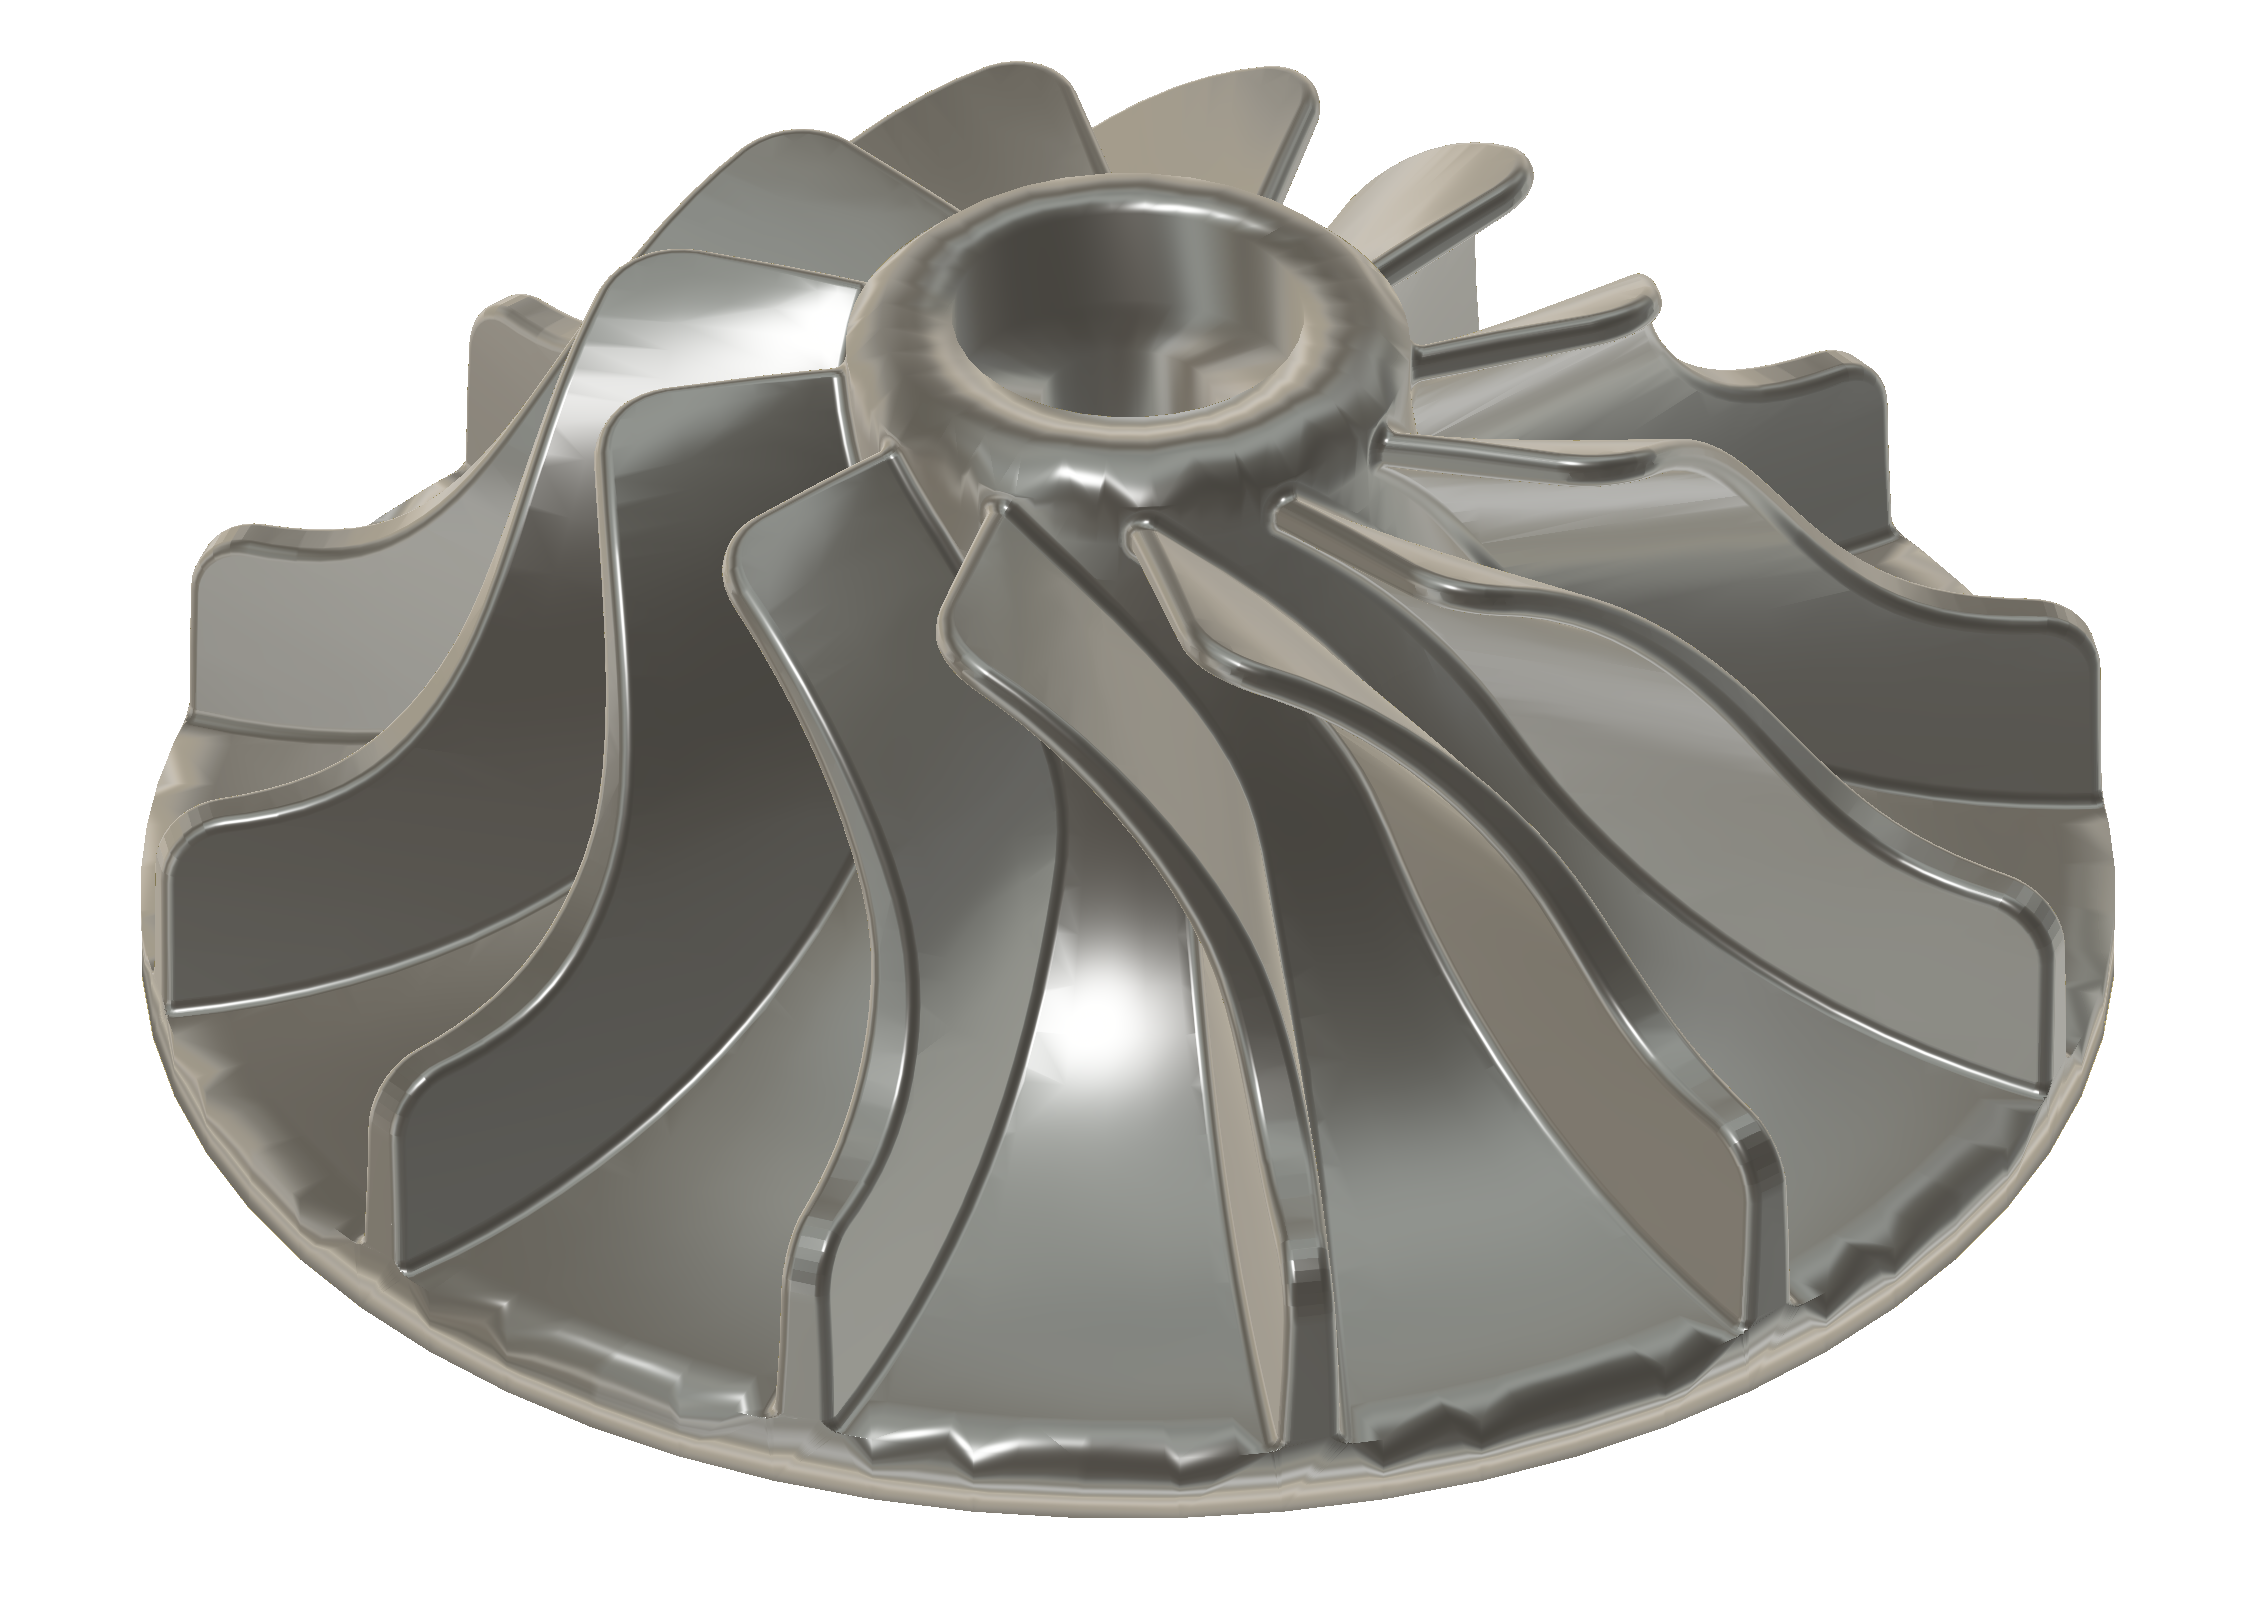
\includegraphics[height=2.8cm]{figs/turbine.png}
    }
    \hfill{}
    \subfloat[Gear \parencite{karlie2018}]{
        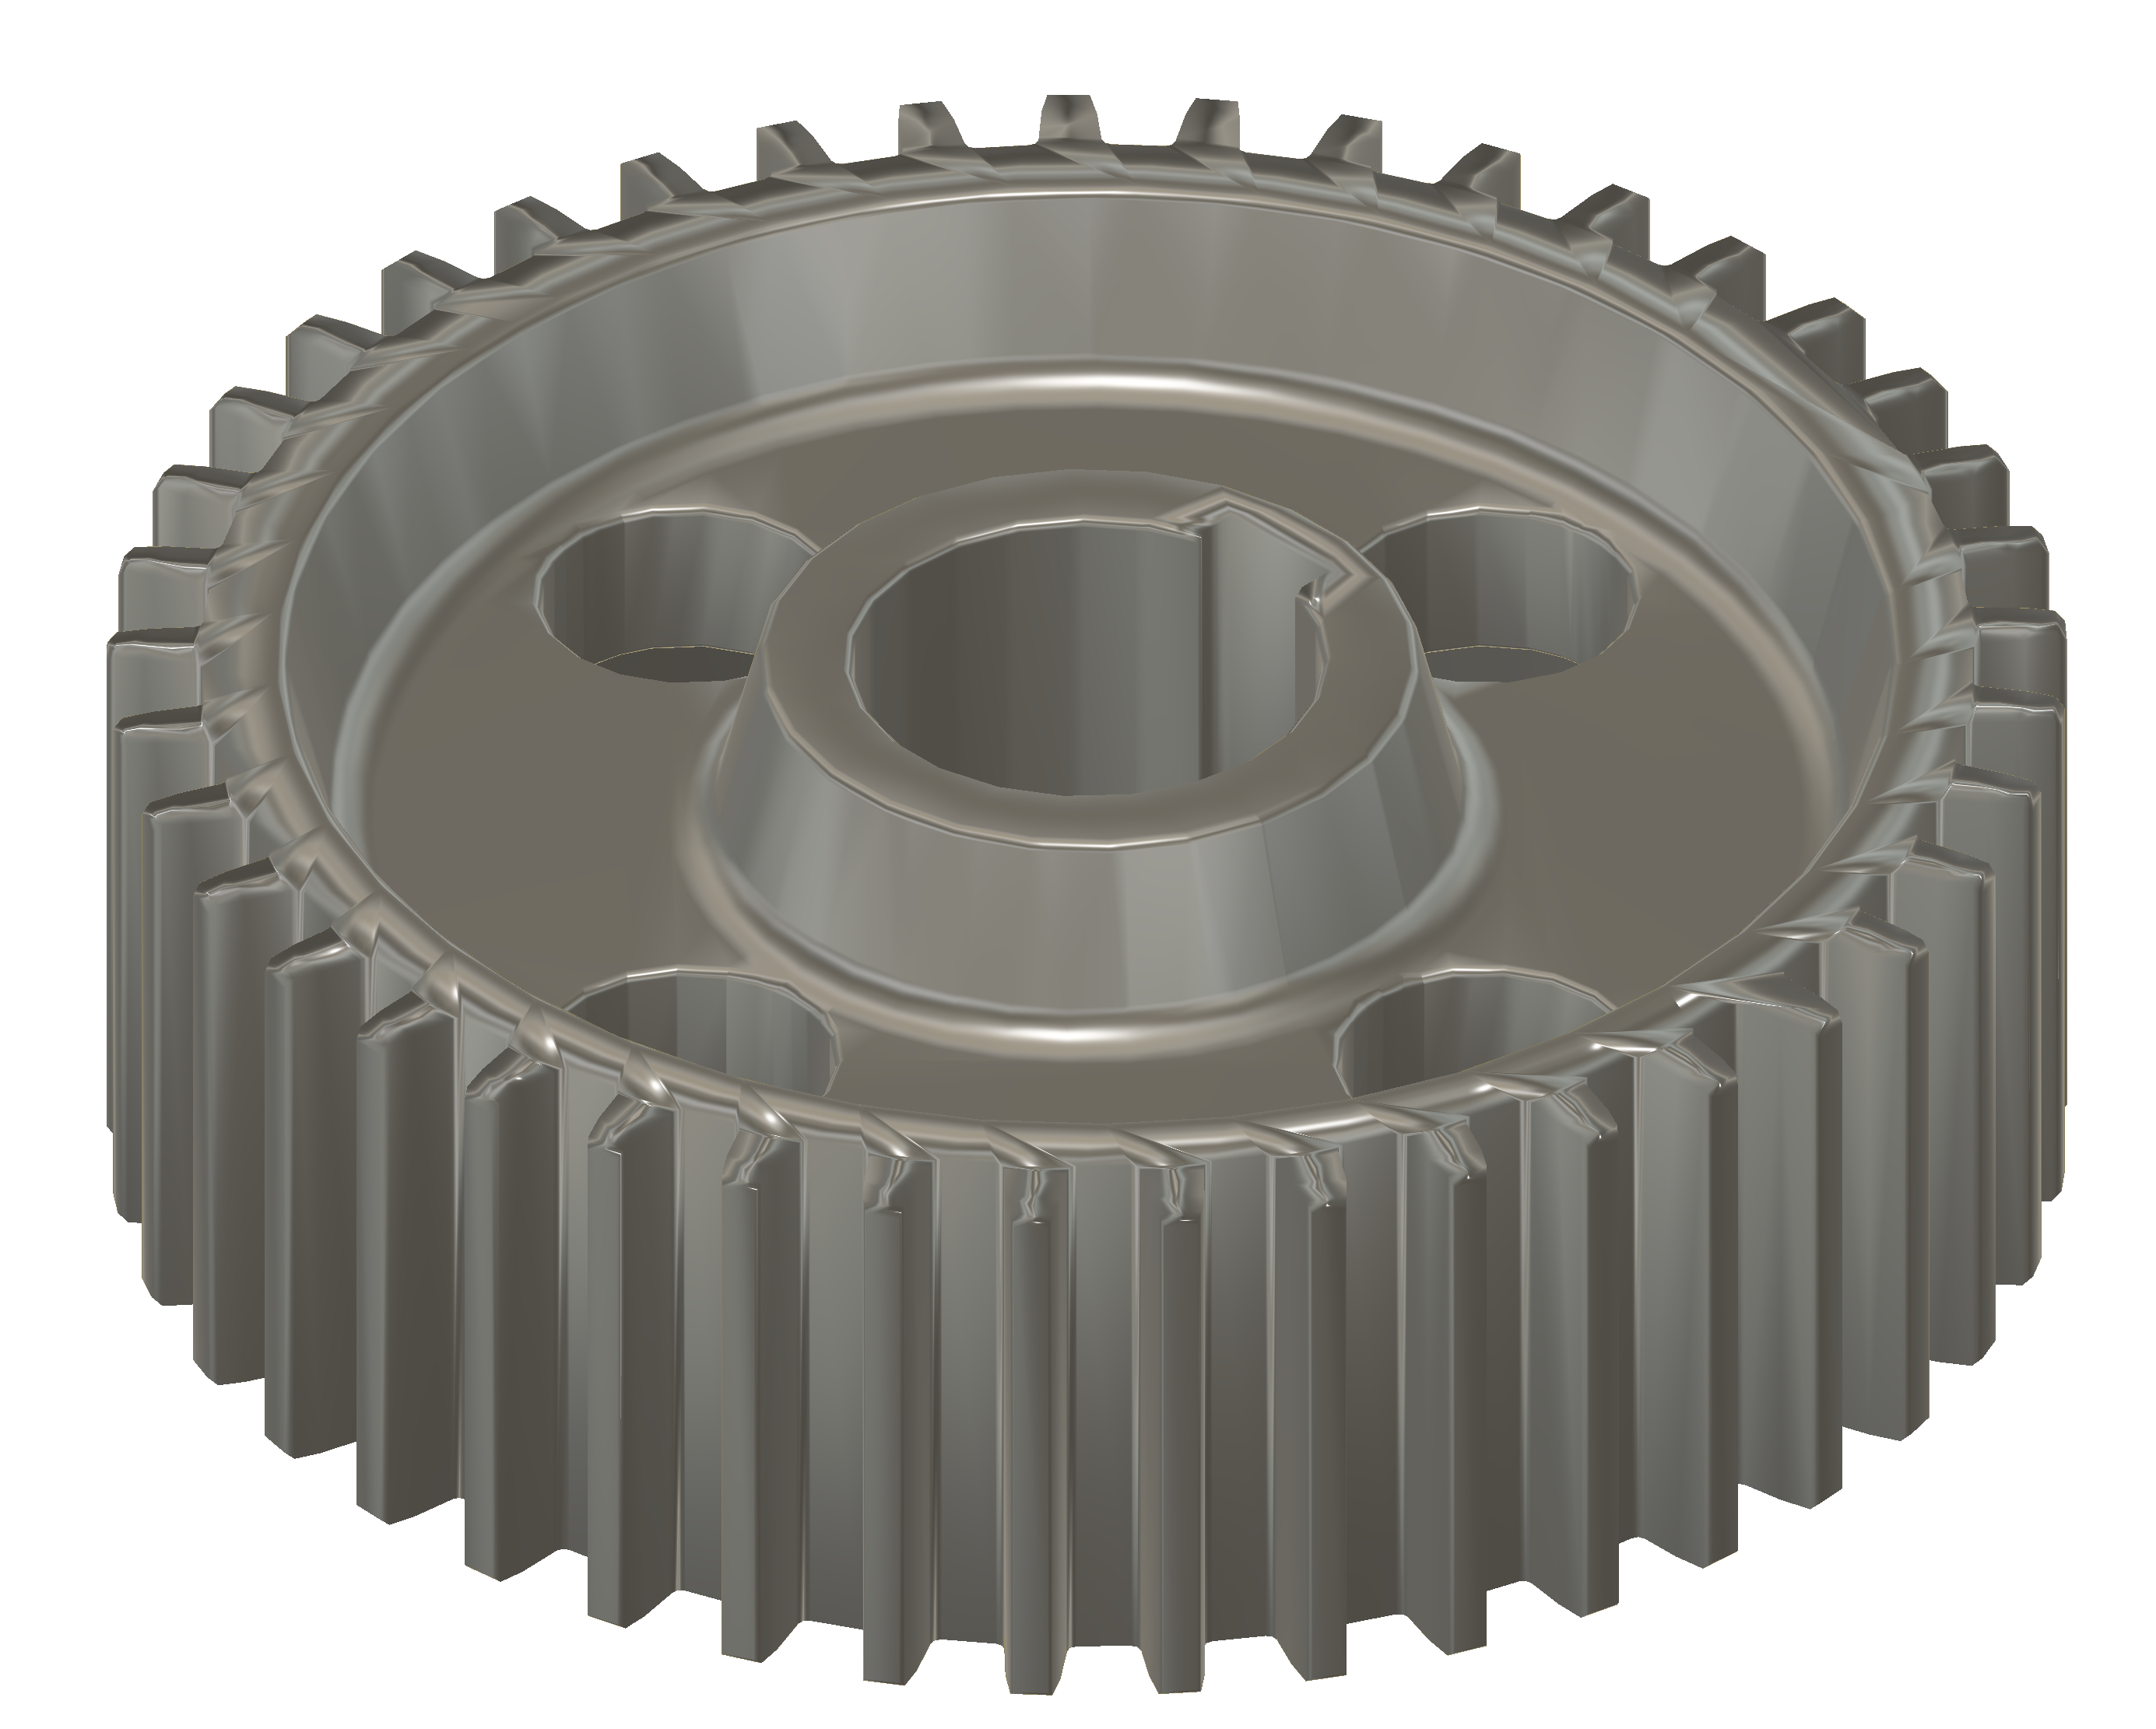
\includegraphics[height=2.8cm]{figs/gear.png}
    }
    \hfill{}
    
    \leavevmode \\
    
    \hfill{}
    \subfloat[Car~\cite{amagliani2018}]{
        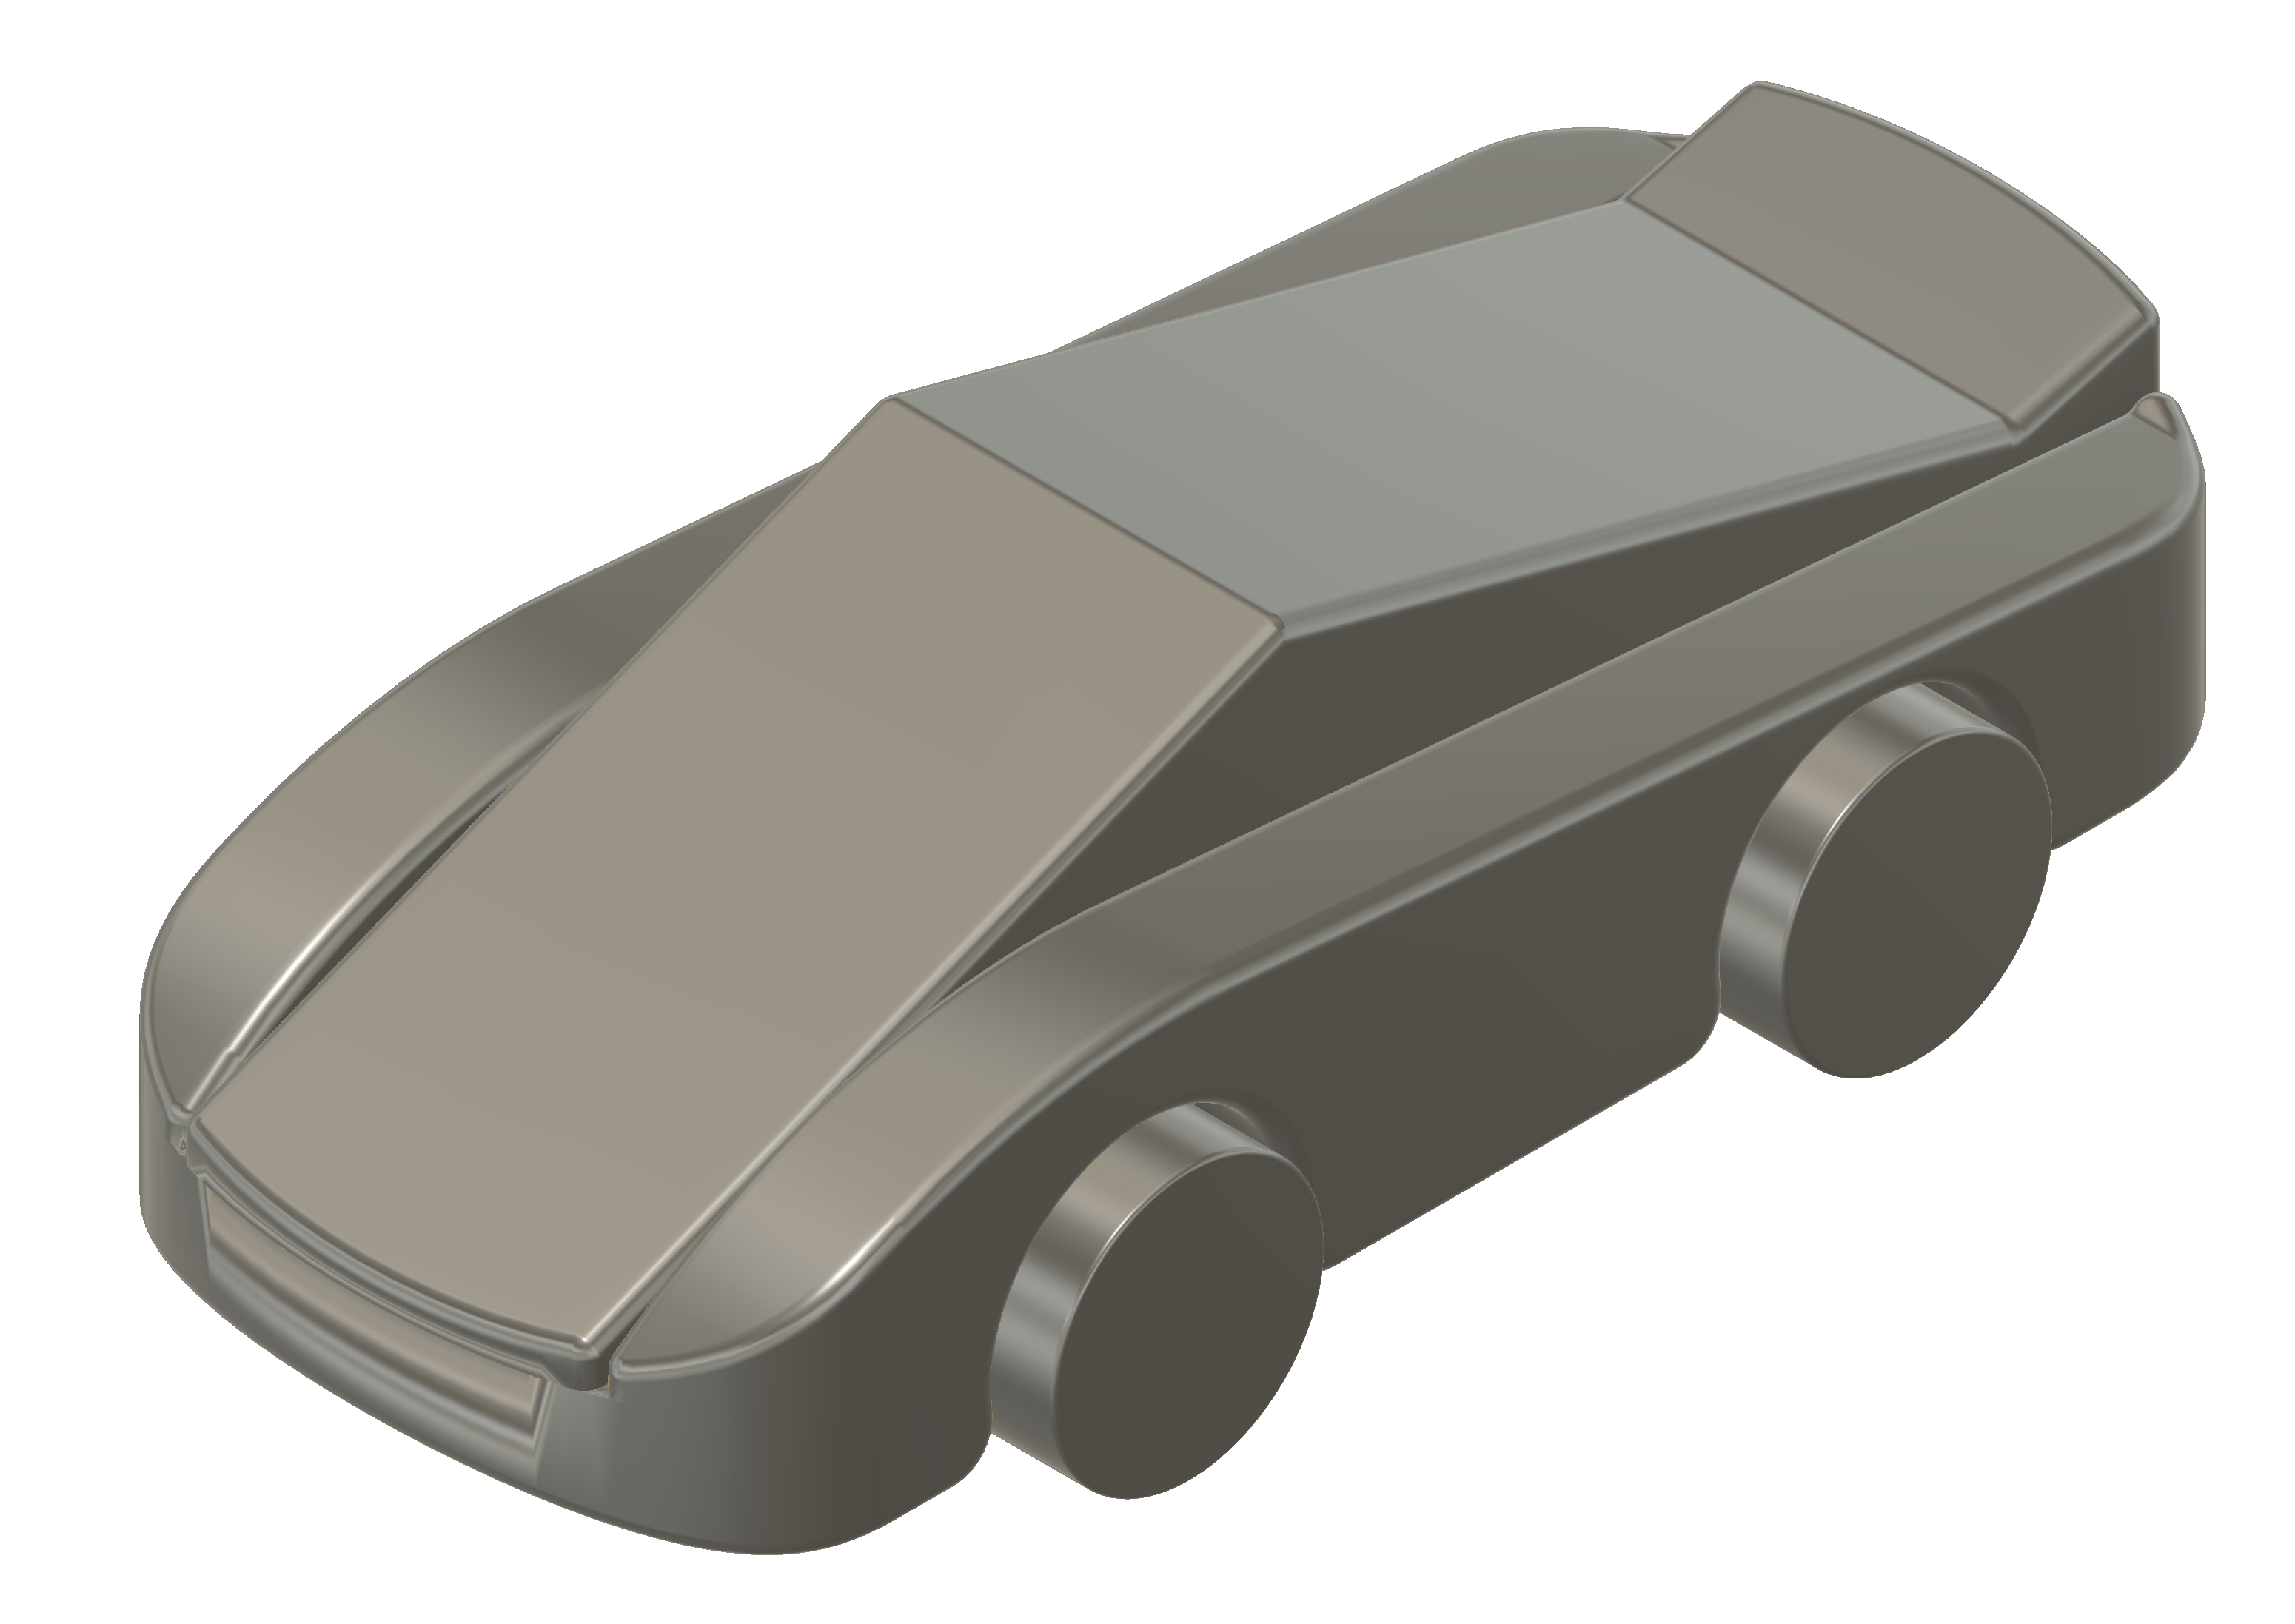
\includegraphics[height=2.8cm]{figs/car.png}
        \label{fig:car}
    }
    \hfill{}
    \subfloat[Mouse~\cite{patil2018}]{
        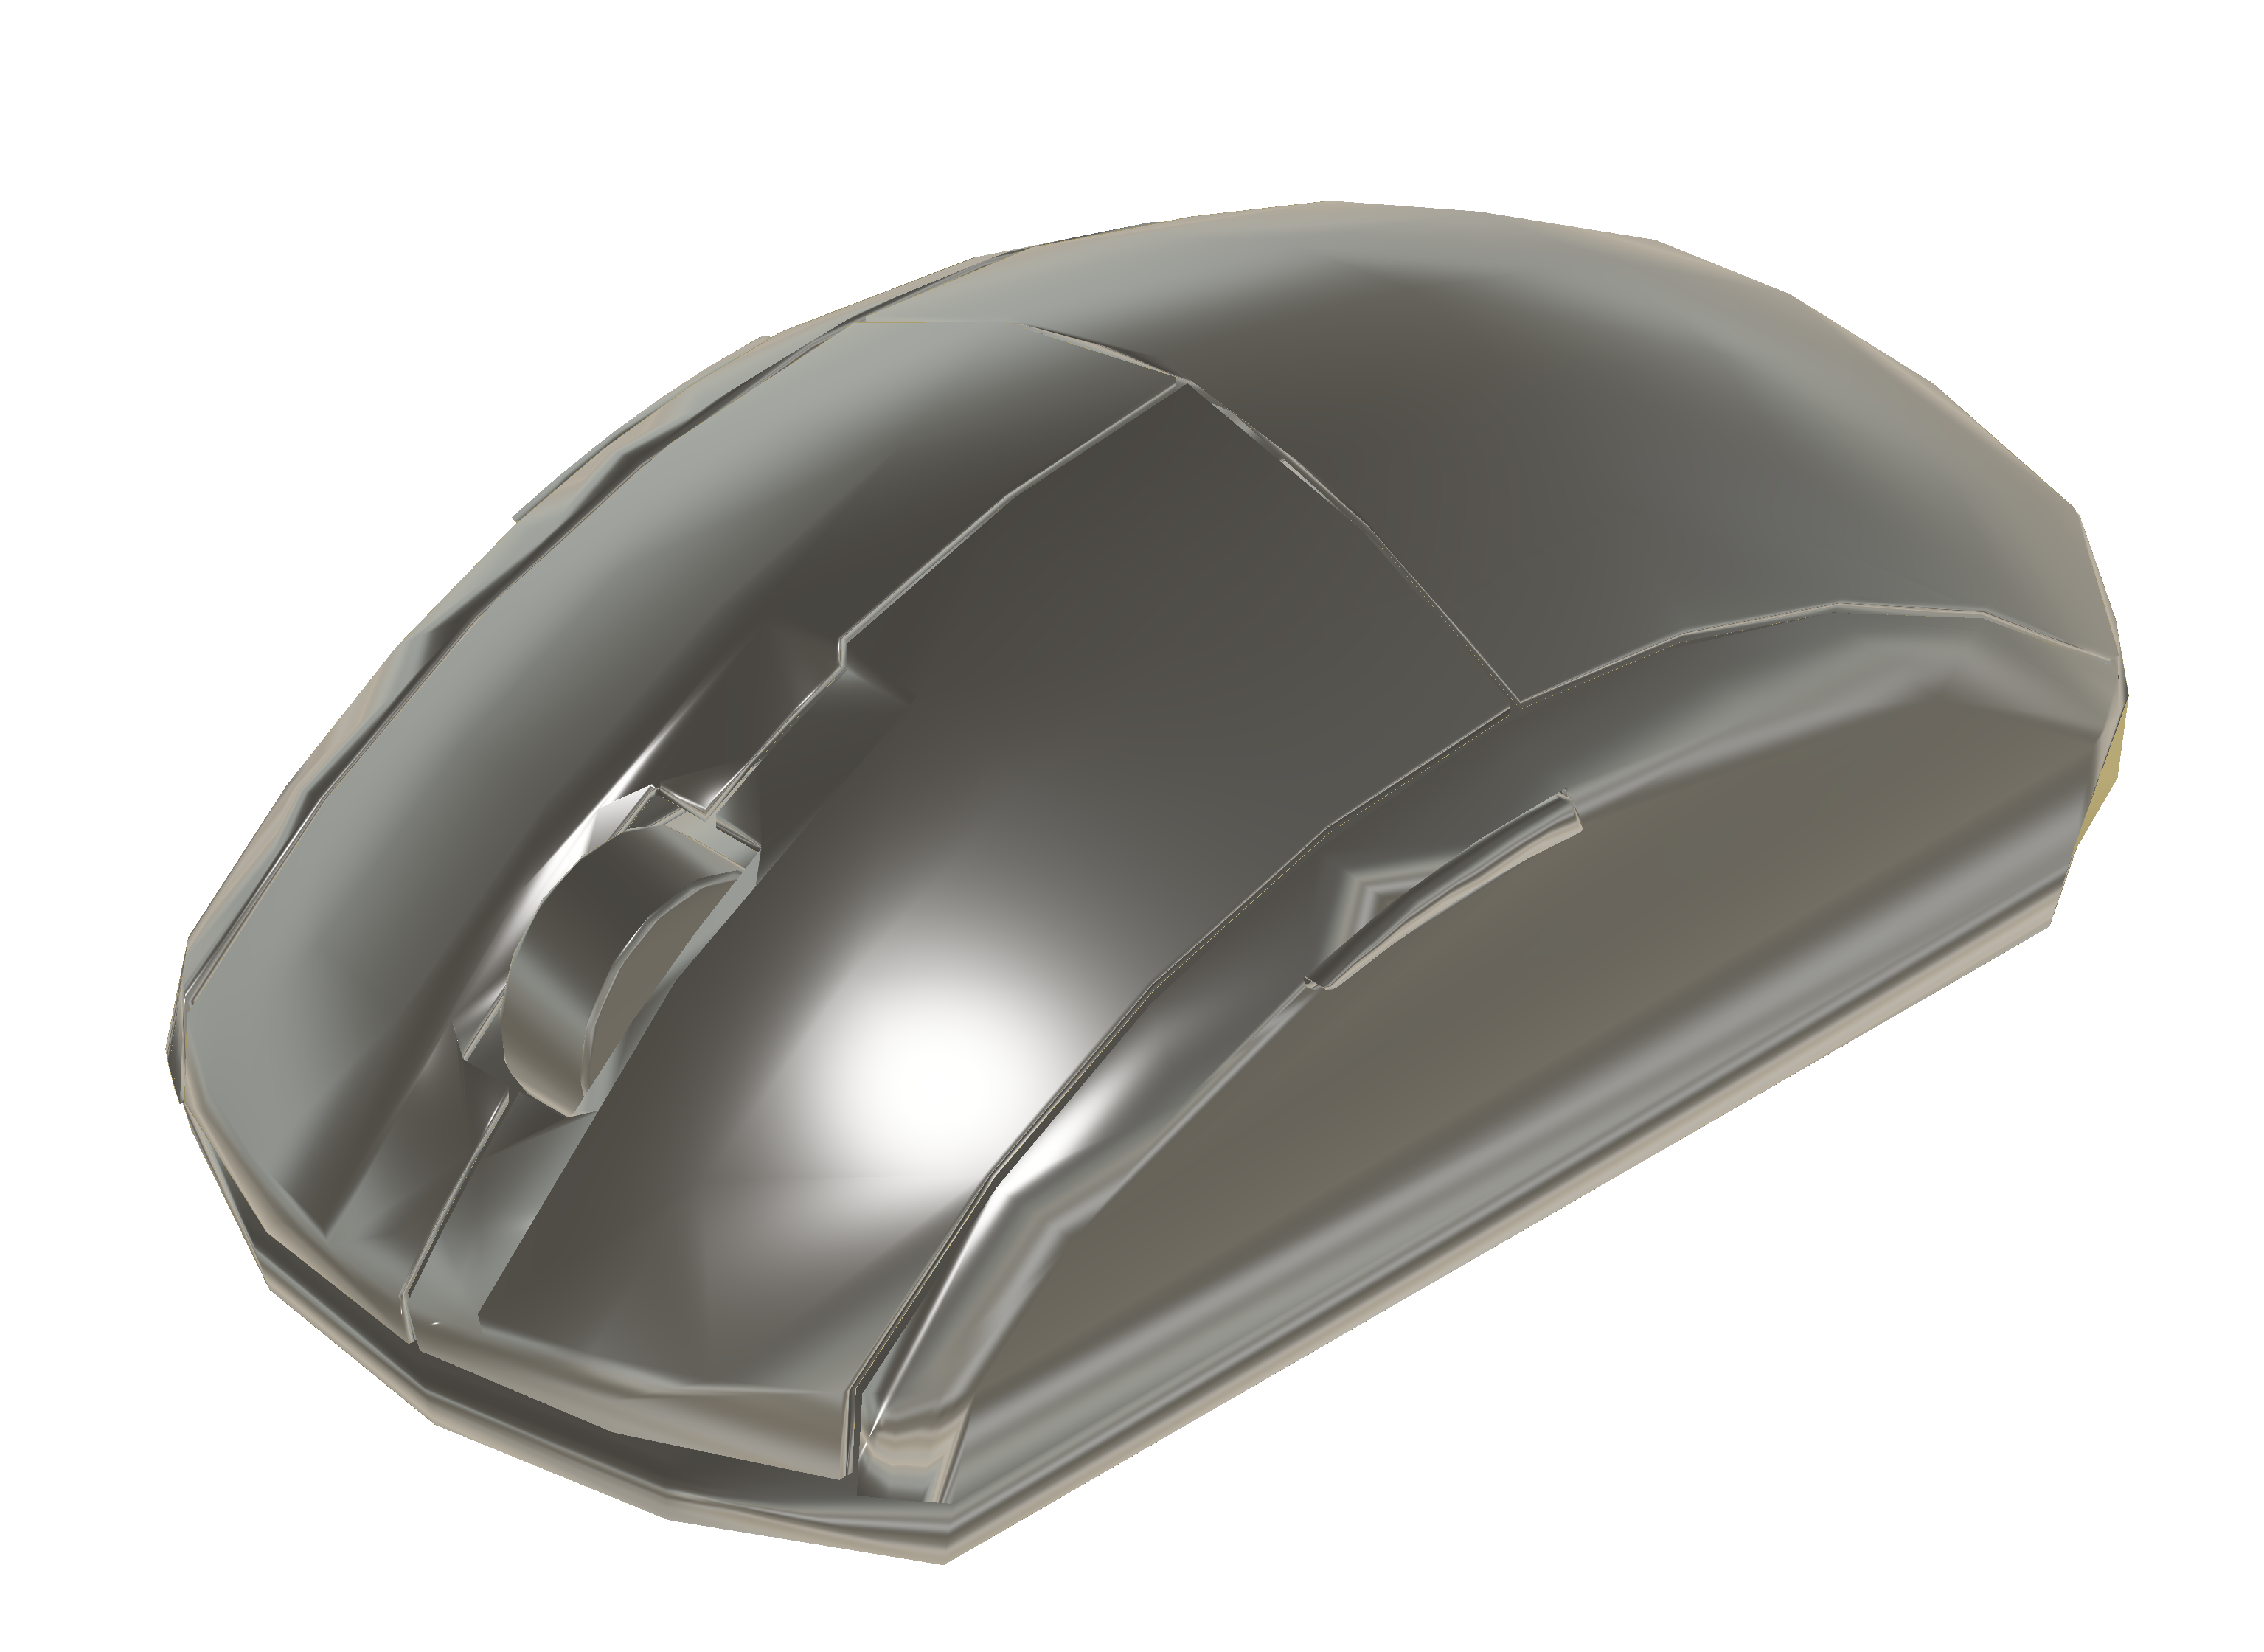
\includegraphics[height=2.8cm]{figs/mouse.png}
        \label{fig:mouse}
    }
    \hfill{}
    
    \caption{Models selected from GrabCAD}\label{fig:cad-models}
\end{figure}

\subsection{Generating the surrogate model}

To generate the surrogate model, the models (in STL format) were placed in Blender and $500 \times 500$ pixel renders produced at \ang{6} increments rotating about the $y$ and $z$ axes (\cref{fig:render-a}). The scene has been set-up to mimic a lightbox in order to emphasise the geometric features and patterns of the models and normalise the background. This was validated against a real-world lightbox scene through linear intensity correlation using the Pearson Correlation Coefficient and colour distribution closeness using Bhattacharyya distance. This resulted in a set of rendered images labelled against the CAD models (\cref{fig:render-b}). The rendering time for the 915 image dataset was \SI{4.1}{\hour}.

\begin{figure}[t!]

    \hfill{}
    \subfloat[Rendering the object in \ang{6} increments]{
        \includestandalone[height=5cm]{standalone/render-capture}
        \label{fig:render-a}
    }
    \hfill{}
    \subfloat[Collage of renders]{
        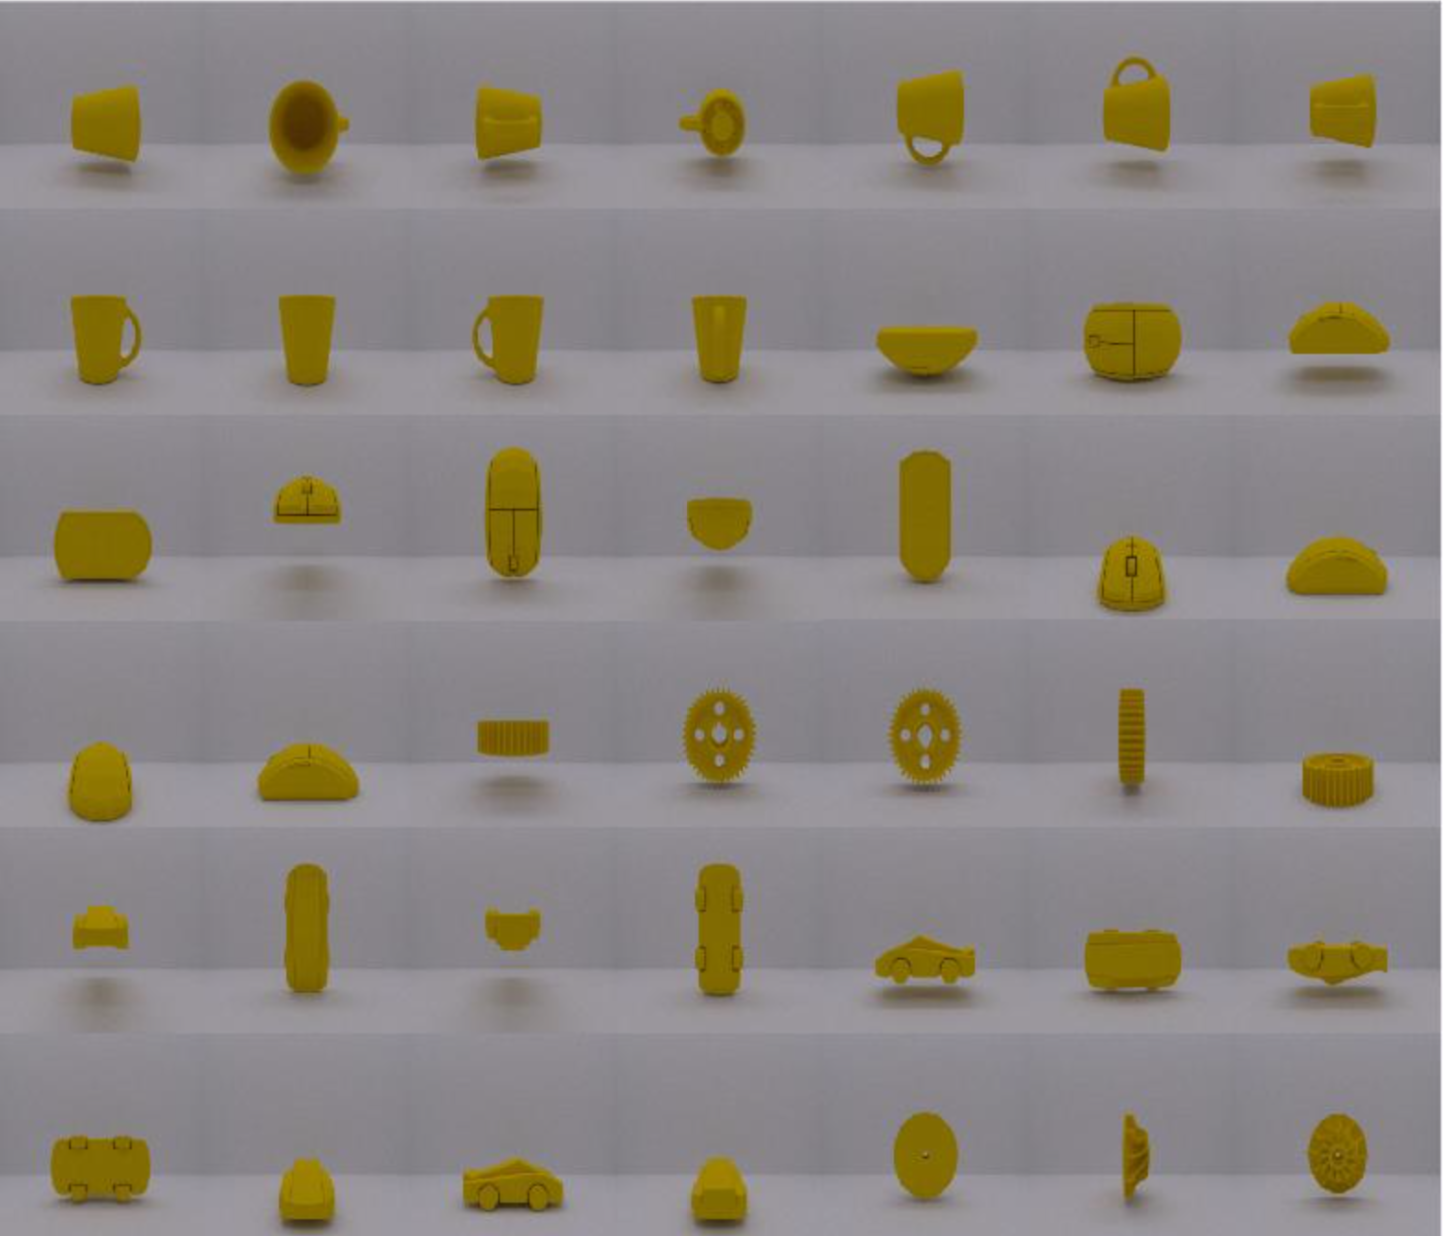
\includegraphics[height=5cm]{figs/renders.png}
        \label{fig:render-b}
    }
    \hfill{}
    \caption{Rendering the object in \ang{6} increments}\label{fig:render-points}
\end{figure}

\subsection{Train}

With the surrogate model generated, the study moved to training the CNN.
Five CNNs were selected to investigate the influence of the CNN architecture on the accuracy and computational requirements.
This also ensures that the particular implementation does not skew the findings in evaluating the potential of CNNs as an approach for CAD model to real-world image classification.
The CNNs are described in Table 2 and have been developed to be trained on labelled images having all performed well in CNN competitions, such as ImageNet.
For each model, the surrogate model renders where re-scaled to the required input size.

The CNN training, validation and testing applied the well-established 80\% training, 10\% validation and 10\% testing.
In this case, the training and validation images come from the surrogate model and testing from real-world images of 3D-printed versions of the CAD models.
Training was left until 200 iterations were complete.

\begin{table}
    \centering
    \caption{CNNs evaluated}\small
    \begin{tabular}{l r r r r}
    \toprule
        Network & Depth & Size [MB] & Parameters [M] & Input Size \\
    \midrule
        AlexNet \parencite{alexnet} & 8 & 227 & 61.0 & 227x227 \\
        GoogleNet \parencite{googlenet} & 22 & 27 & 7.0 & 224x224 \\
        ResNet-18 \parencite{resnet} & 18 & 44 & 11.7 & 224x224 \\
        ResNet-50 \parencite{resnet} & 50 & 96 & 25.6 & 224x224 \\
        Inception-v3 \parencite{inception} & 48 & 89 & 23.9 & 299x299 \\
    \bottomrule
    \end{tabular}
\end{table}


\subsection{Test \& refine}\label{sec:test}

Having trained the CNNs, three experiments were performed to evaluate the potential in using a surrogate model CNN for real-world object to CAD model classification. The image test used consisted of images taken in a controlled lightbox environment featuring 3D printed versions of the CAD models and totalled 48 images (\cref{fig:real-world}). Images were taken using an iPhone 6 rear-camera which has a 7.99 MP resolution, image sensor size of $4.8 \times \SI{3.6}{\milli\metre^2}$, focal length of \SI{4.15}{\milli\metre} and field of view of \ang{72.8}. The selection of a phone camera reflects the typical type of camera that would be used by the target audience of this model.

The first experiment compares the trained CNNs performance in relation to accurately determining the model captured in the real-world images. The second experiment investigates the potential in augmenting the surrogate model to investigate how the accuracy can be improved with minimum additional computational cost and the compromise that could be made between render time and CNN accuracy. The third and final experiment sought to understand how reducing the number of renders in the surrogate model effects the accuracy of the CNN.

\begin{figure}[t!]
    \centering
    \subfloat[Car]{
        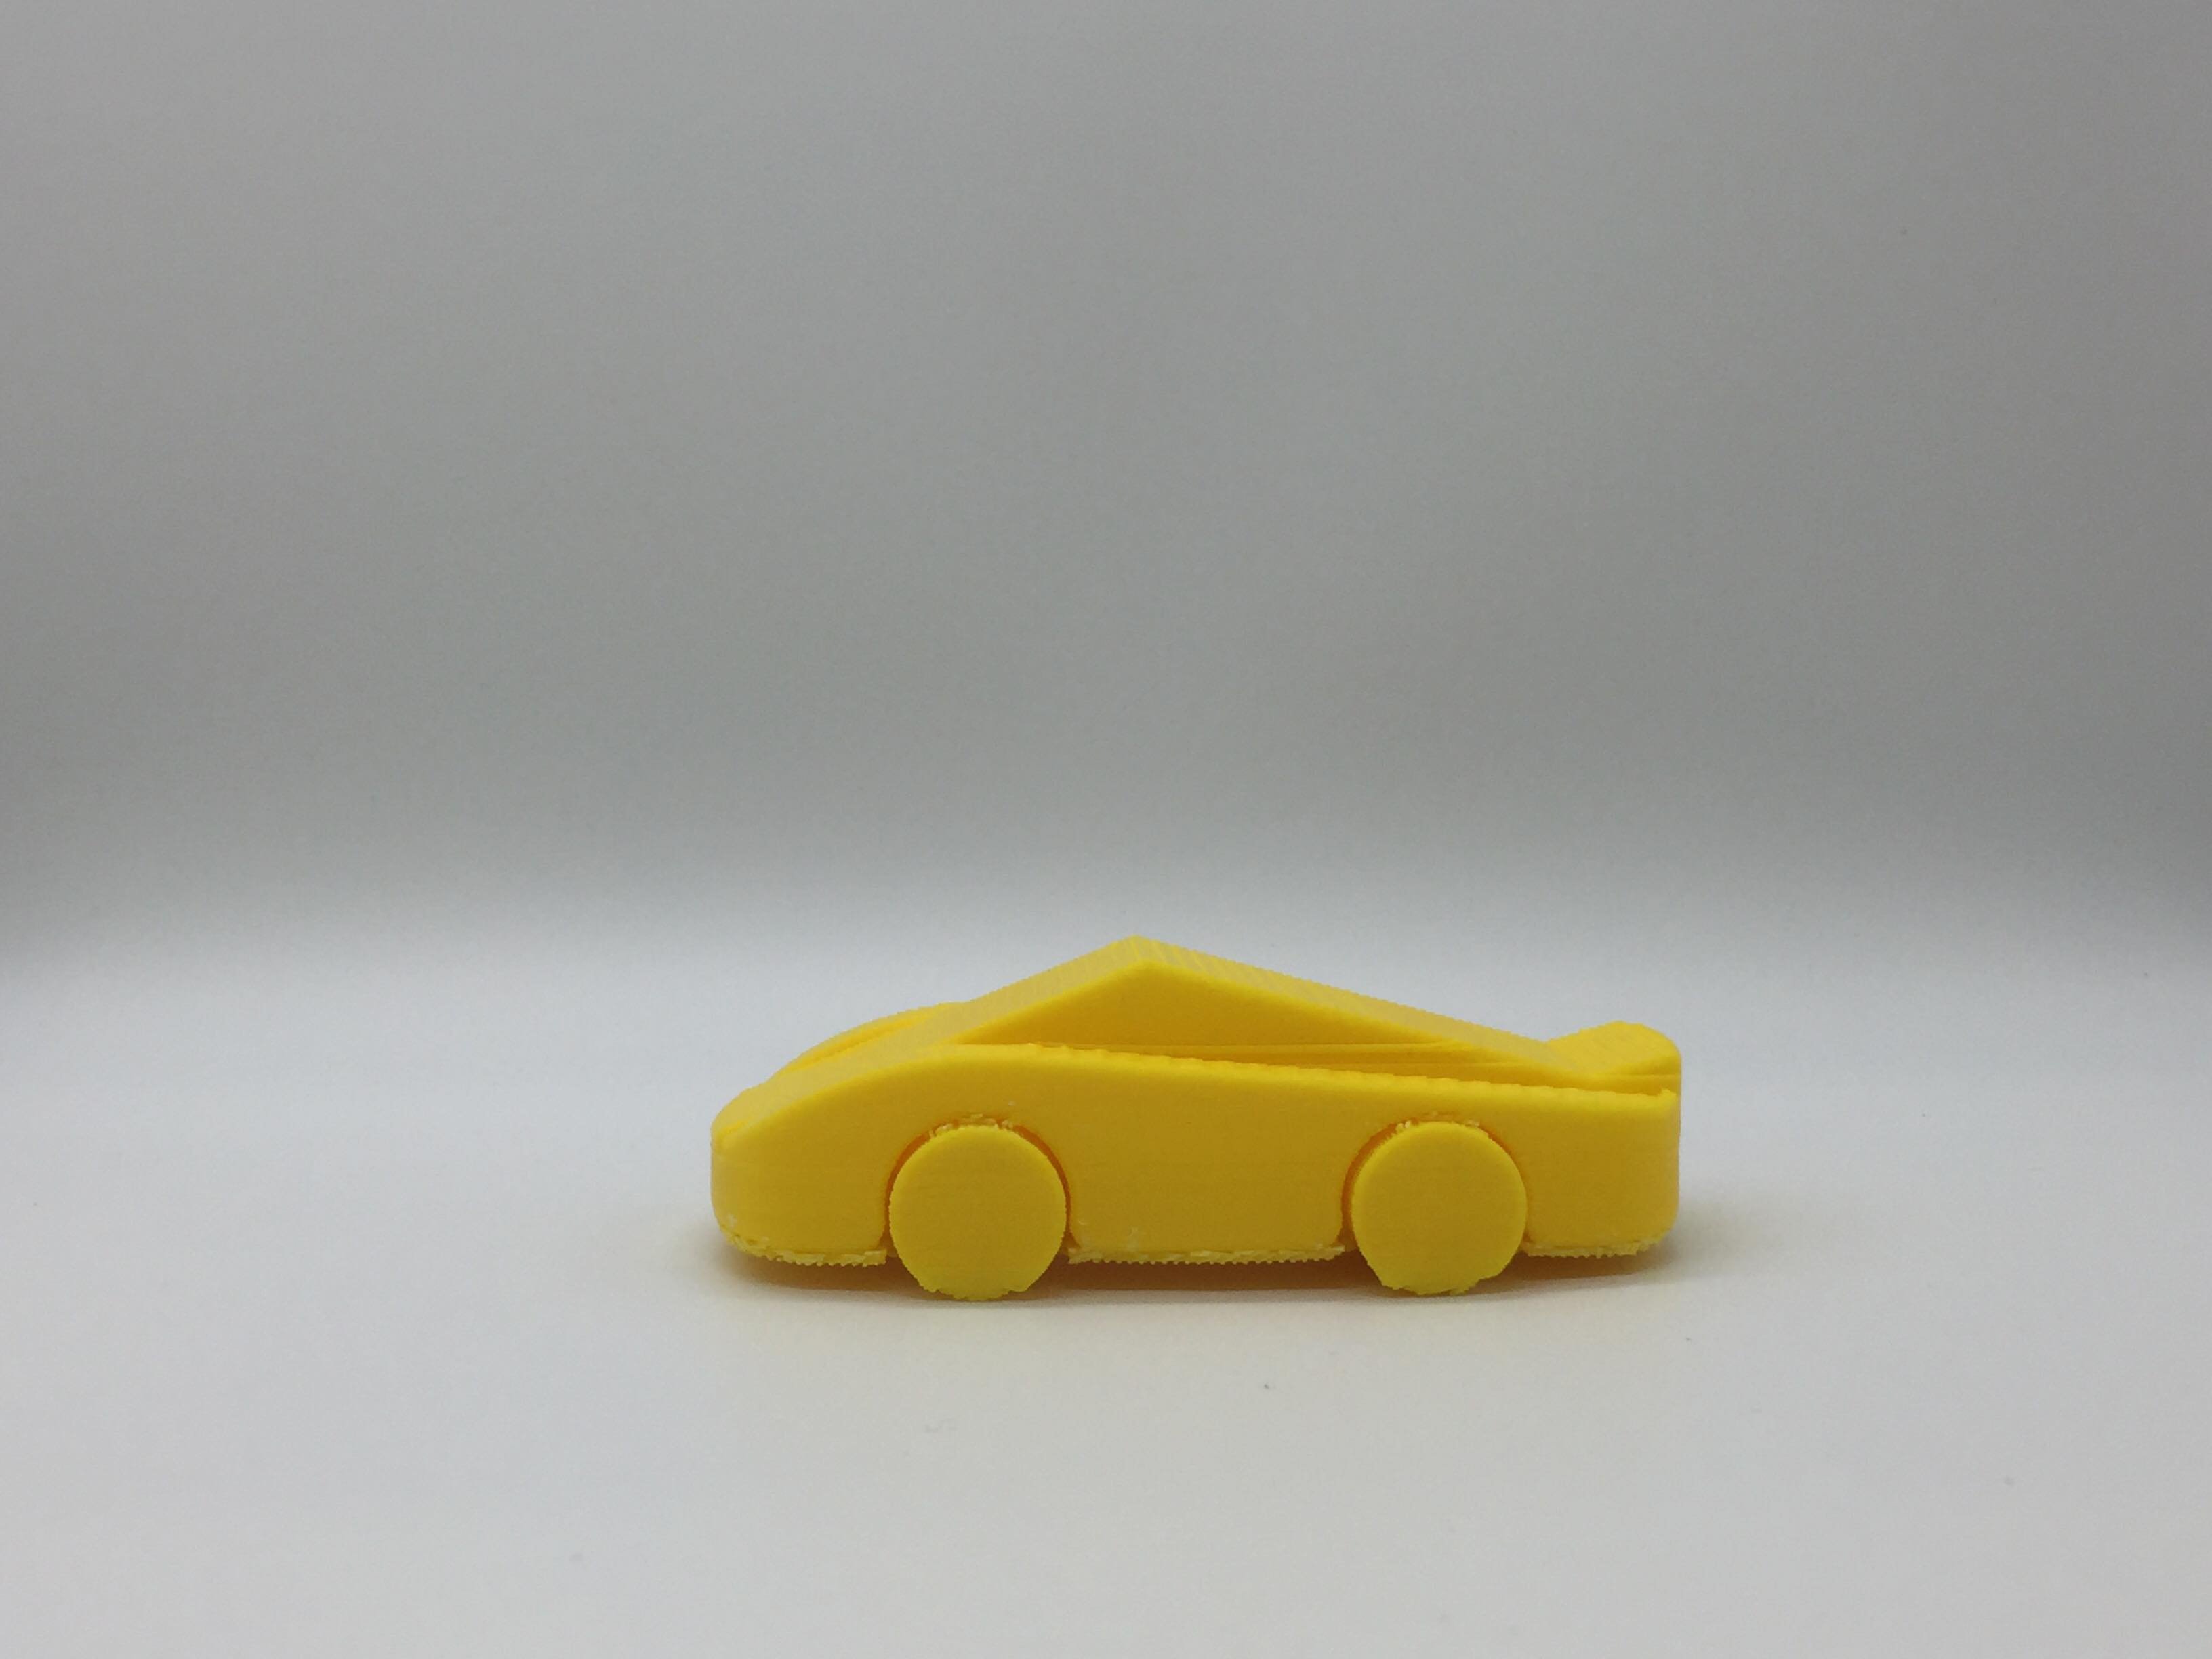
\includegraphics[width=0.3\textwidth]{figs/real-car-photo.jpg}
    }
    \hfill 
    \subfloat[Gear]{
        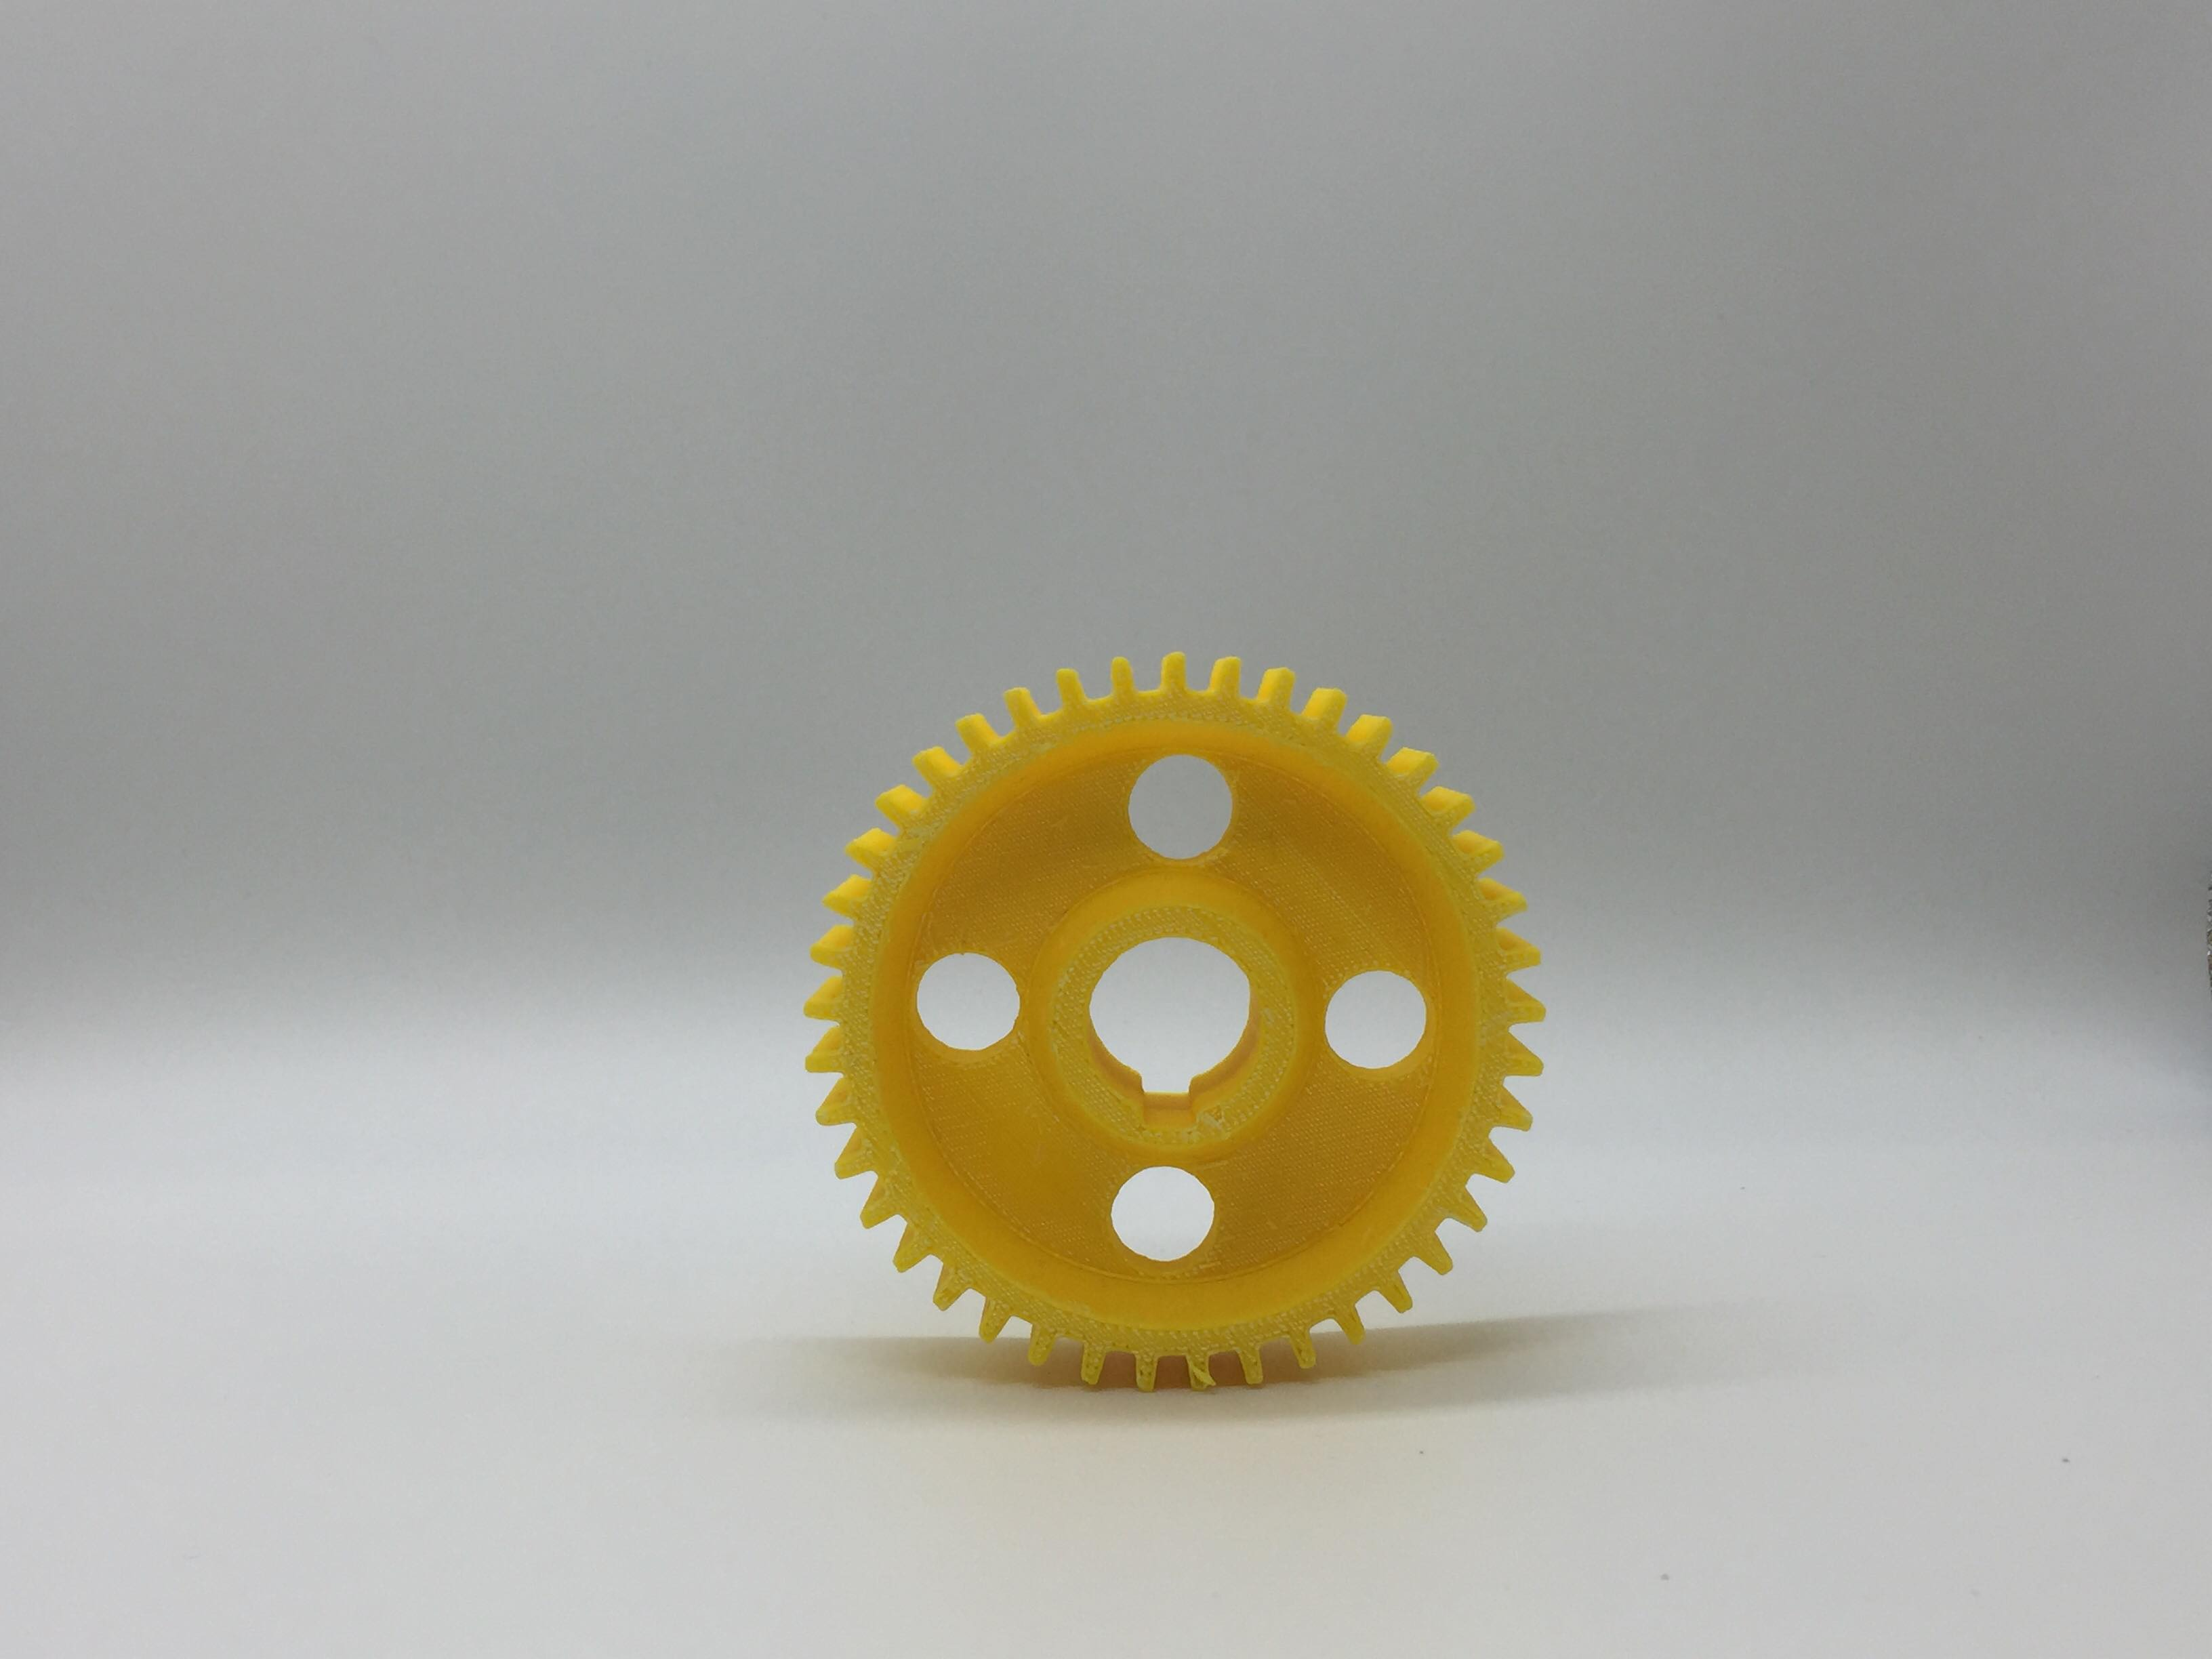
\includegraphics[width=0.3\textwidth]{figs/real-gear.jpg}
    }
    \hfill 
    \subfloat[Mouse]{
        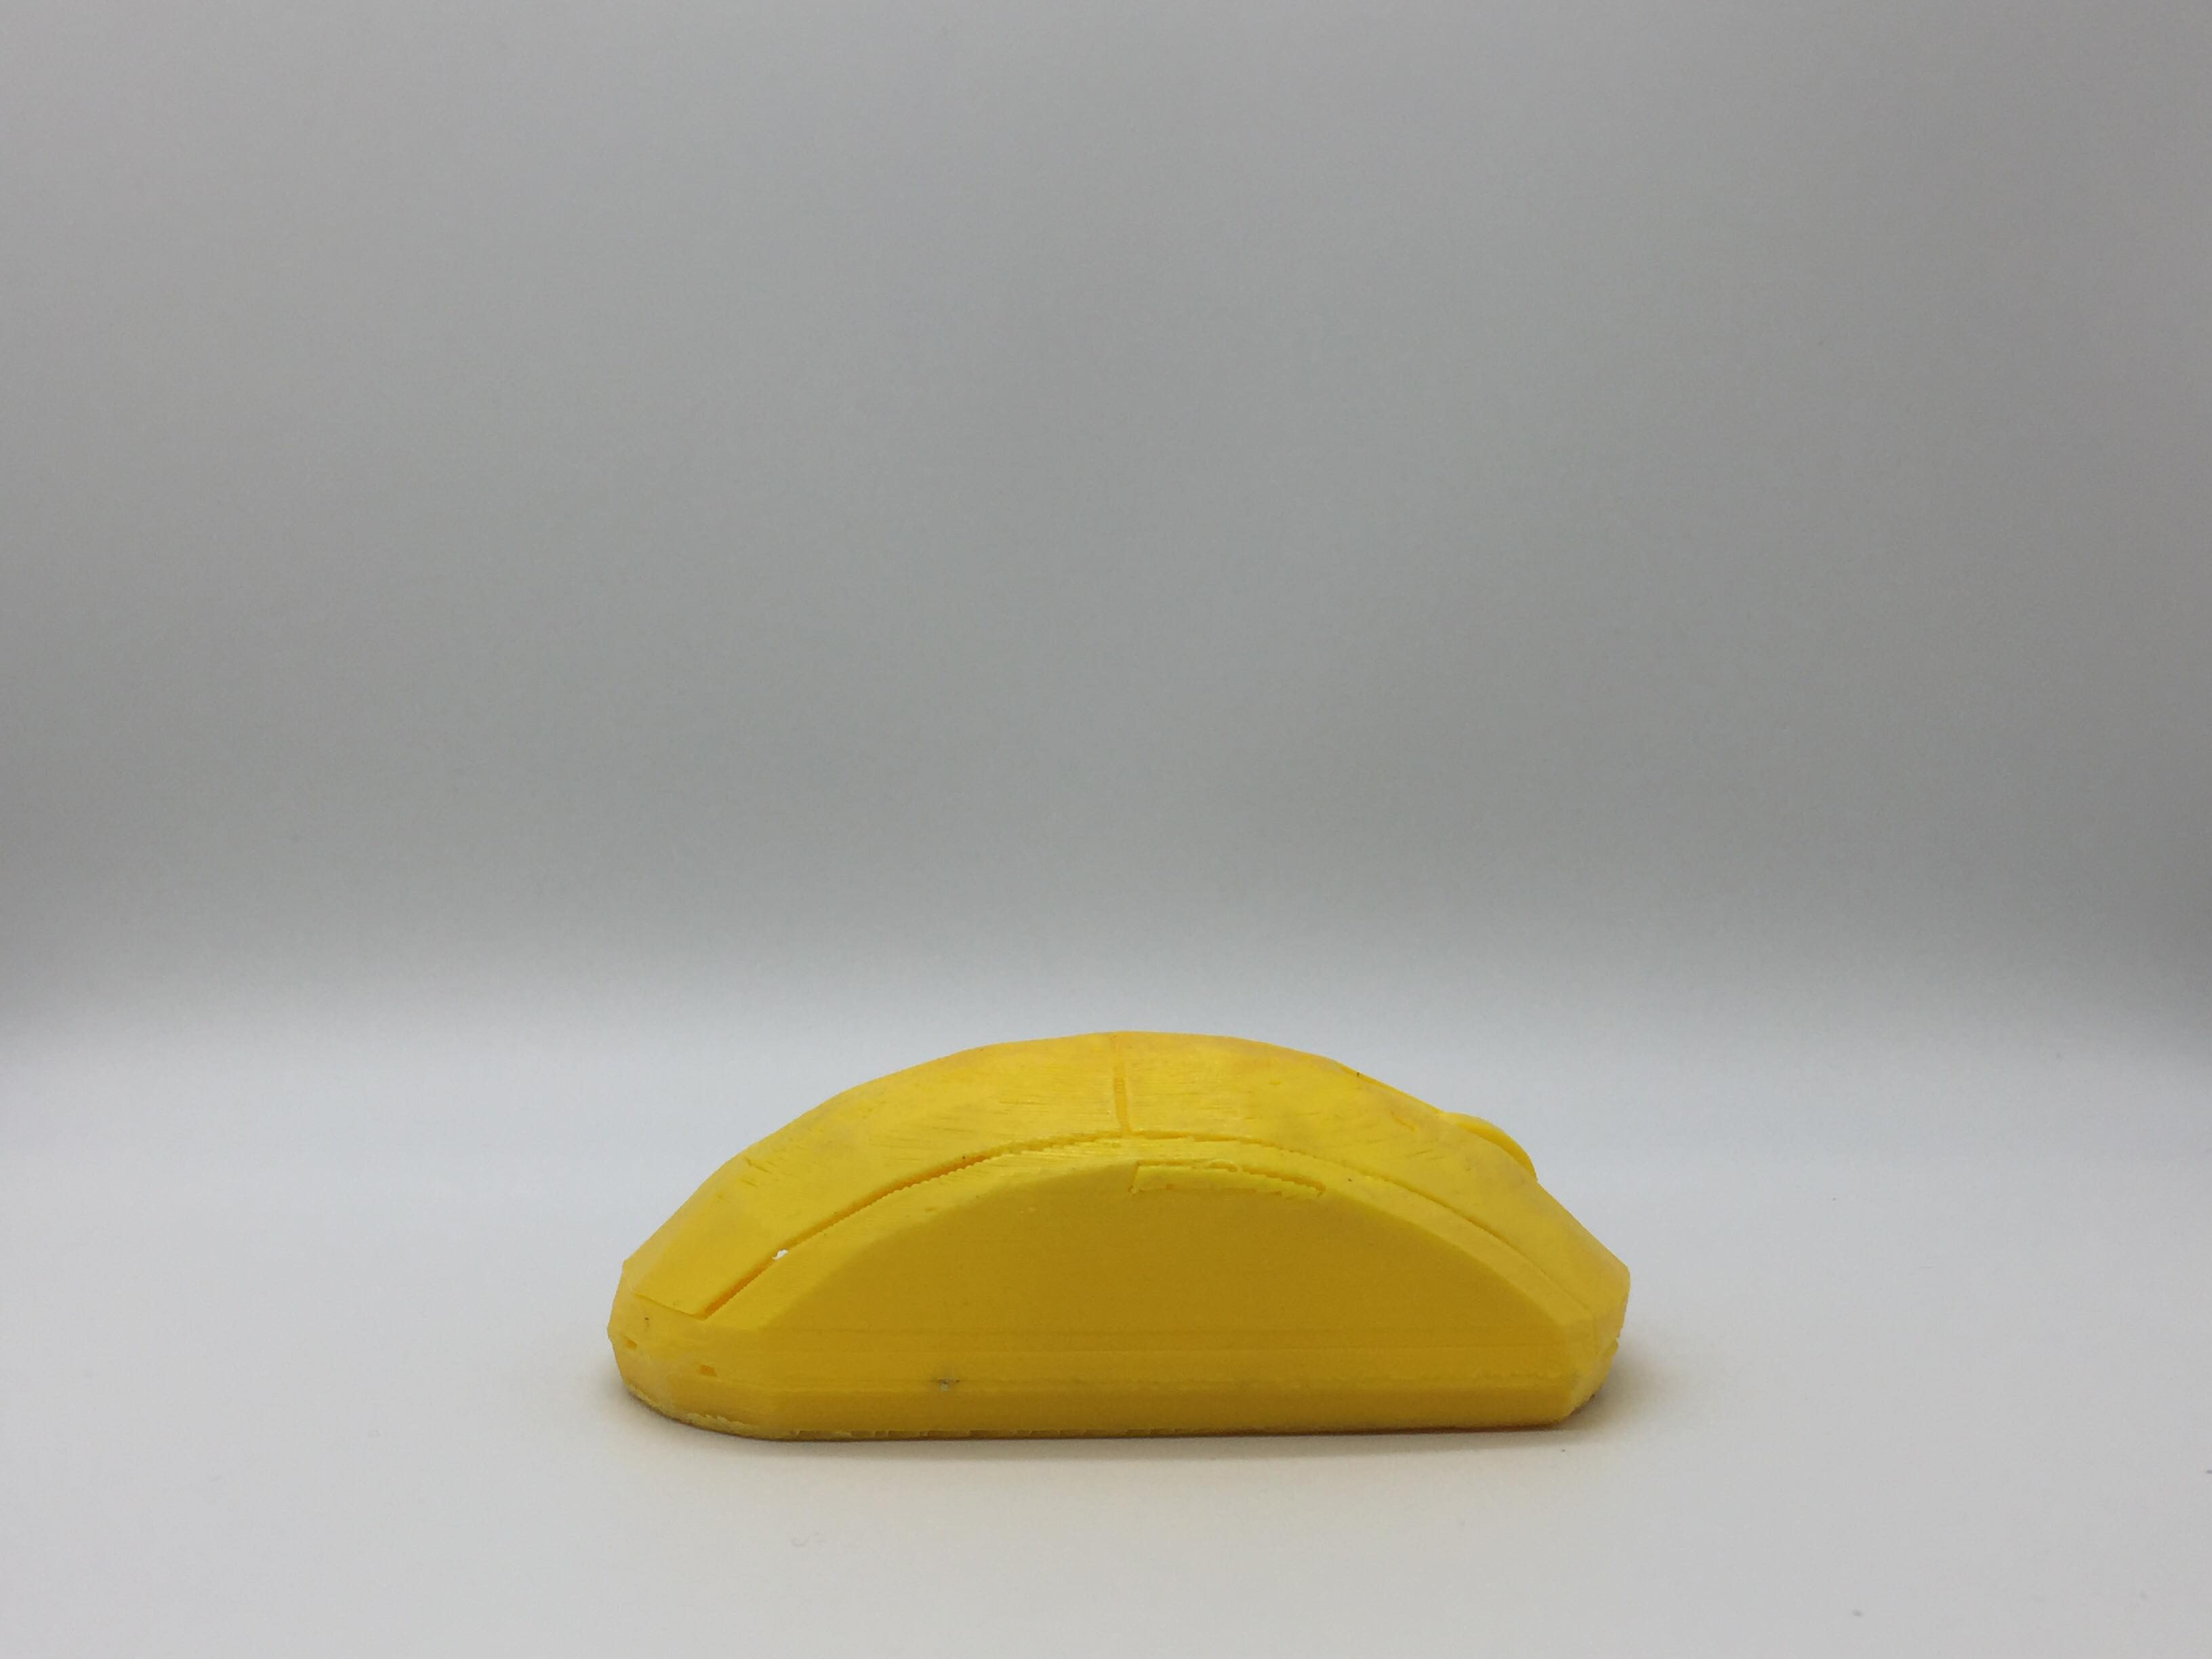
\includegraphics[width=0.3\textwidth]{figs/real-mouse.jpg}
    } 
    \caption{Real-world photograph of 3d-printed models}\label{fig:real-world}
\end{figure}


\section{Results}\label{sec:res}

This section details the results of the three experiments outlined in \cref{sec:test}.

\subsection{Experiment 1. CNN comparison}

\cref{tbl:acc} details the performance results for the 5 CNNs trained on the surrogate model and tested against real-world photos. It can be seen that both AlexNet and GoogleNet perform well in identifying real-world images even though they were trained on a surrogate model. This confirms that a surrogate model approach is viable for the classification of objects. Further, the associated mean confidence scores for correctly and incorrectly labelled images shows that the CNNs confidence value can be used as a threshold to prevent false positive detection.

However, the ResNet and Inception models did not perform as well even though they outperform AlexNet and GoogleNet in the ImageNet tests. They also require significantly greater training time. This reveals the importance of the CNN architecture for the given application.

From these results, AlexNet was selected as the CNN to carry forward to Experiment 2 due to its low training time and high accuracy. The accuracy of 83.3\% also provided headroom to evaluate the capability of augmentation to support the training of the CNNs.

\begin{table}
  \centering
  \caption{CNN accuracy}\label{tbl:acc}
  \footnotesize
  \begin{tabular}{l R{2.2cm} r R{2cm} r r}
    \toprule
      CNN & Training Time [s] & Accuracy [\%] & Correct/ Incorrect & \multicolumn{2}{c}{Mean Confidence [\%]} \\
      & & & & Correct & Incorrect \\
      \midrule
      AlexNet & 680 & 83.3 & 40/8 & 89.4 & 68.9 \\
      GoogleNet & 1914 & 91.7 & 44/4 & 88.6 & 63.4 \\
      ResNet-18 & 1553 & 27.1 & 13/35 & 34.2 & 32.7 \\
      ResNet-50 & 4949 & 33.3 & 16/32 & 39.0 & 38.4 \\
      Inceptionv3 & 7160 & 22.9 & 11/37 & 25.7 & 23.0 \\
    \bottomrule
  \end{tabular}
\end{table}

\subsection{Experiment 2. Augmentation}

Augmentation is the process of manipulating the input images in order to increase the training set size through methods of low-computational cost~\cite{Mikołajczyk}. The first method is rotation of the image about its centre. Both \ang{90} and \ang{180} were trialled with \ang{90} increasing the accuracy of AlexNet to 96.2\%. However, this is at the detriment of the difference in confidence measures between correct and incorrect results (\cref{tbl:aug}). This would lead to the tool providing a greater number of accurate results but with a greater likelihood of false positives.

The second method is reflection, which was performed about the $x=0$ and $y=0$ axes of the image. \cref{tbl:aug} reveals that all forms of reflection improved the accuracy of AlexNet with x, y giving the greatest increase in accuracy while also maintaining a significant difference between the mean correct and incorrect confidence scores enabling false positive detection.

The third method trialled was scaling of the image through the ranges of 0.9–1.1, 0.8–1.2 and 0.7–1.3. The centre of the image was the point at which the scaling was acted upon. This yielded results similar to reflection where an increase in accuracy while maintaining the difference in confidence values was preserved.

From these results, it was decided to continue with AlexNet trained on a surrogate model that had been augmented through reflection by $x$, $y$.

\begin{table}[t!]
  \centering
  \caption{Effect of augmentation on the predictive power of the CNN}\label{tbl:aug}\small
  \begin{tabular}{l r r r}
    \toprule
      Test Data & Accuracy [\%] & \multicolumn{2}{c}{Mean Confidence [\%]} \\
      & & Correct & Incorrect \\
    \midrule
      Original & 83.3 & 80.0 & 51.0 \\
    \midrule
      \multicolumn{4}{l}{Rotation} \\
    \midrule
      $\pm\ang{90}$ & 96.2 & 94.5 & 82.5 \\
      $\pm\ang{180}$ & 89.7 & 94.9 & 69.3 \\
    \midrule
      \multicolumn{4}{l}{Reflection} \\
    \midrule
      $x$ & 85.9 & 93.1 & 71.0 \\
      $y$ & 89.7 & 93.6 & 92.2 \\
      $x,y$ & 94.9 & 93.5 & 63.7 \\
    \midrule
      \multicolumn{4}{l}{Scaling} \\
    \midrule
      0.9 -- 1.1 & 94.9 & 94.4 & 72.9 \\
      0.8 -- 1.2 & 89.7 & 96.8 & 83.2 \\
      0.7 -- 1.3 & 91.0 & 96.2 & 62.6 \\
    \bottomrule
  \end{tabular}
\end{table}

\subsection{Experiment 3: Reduction}

Experiment 3 investigated the potential in reducing the surrogate model dataset to provide an indication of the minimum level of rendering time that would be required given that one can enhance the dataset through augmentation. \cref{tbl:reduction} presents the results of reducing the surrogate model dataset. It can be seen that an 80\% reduction of the dataset can be achieved with only a 10\% loss in accuracy and 10\% reduction in the margins between confidences. This highlights the potential of using a reduced and less computationally expensive surrogate model dataset, 1.37 h from 4.1 h in render time.

\begin{table}[t!]
  \centering
  \caption{Effect of reduction on the predictive power of the CNN}\label{tbl:reduction}\small
  \begin{tabular}{r r r r}
    \toprule
      Reduction [\%] & Accuracy [\%] & \multicolumn{2}{c}{Mean Confidence [\%]} \\
      & & Correct & Incorrect \\
    \midrule
      00 & 94.9 & 93.5 & 63.7 \\
      20 & 93.6 & 96.5 & 73.0 \\
      50 & 92.3 & 93.9 & 56.9 \\
      80 & 84.6 & 91.5 & 72.5 \\
    \bottomrule
  \end{tabular}
\end{table}

\cref{fig:conf} shows the confusion matrices for the four reductions. Confusion matrices visualises the results true to predicted class prediction made by the CNN and enables the identification of common classes that may be confused with one another. Out of the five models used in this study, it reveals that it is the coffee cup and mouse that are often miss-classified and correlates with a lack of, one might argue, features. In contrast, the models with a high number of features, the gear and turbine, are not misclassified until one reaches the 80\% reduction of the surrogate model.

\begin{figure}[t!]

    \hfill{}
    \subfloat[0\%]{
        \includestandalone[width=0.4\textwidth]{standalone/00-percent-reduction}
    }
    \hfill{}
    \subfloat[12\%]{
        \includestandalone[width=0.4\textwidth]{standalone/20-percent-reduction}
    }
    \hfill{}
    
    \leavevmode\\
    
    \hfill{}
    \subfloat[50\%]{
        \includestandalone[width=0.4\textwidth]{standalone/50-percent-reduction}
    }
    \hfill{}
    \subfloat[80\%]{
        \includestandalone[width=0.4\textwidth]{standalone/80-percent-reduction}
    }
    \hfill{}
    
    \caption{Confusion matrices with respect to reducing the size of the surrogate model}\label{fig:conf}
\end{figure}

\section{Discussion and future work}\label{sec:dis}

This study has shown the potential of surrogate model CNNs as a method of classifying real-world images of objects to their respective CAD model, however further work is required to fully realise this and for it to be used on a repository of millions of models. First and foremost is the scaling of these experiments to much larger surrogate models with a greater number of CAD models, as well as increasing the scene variance in the real-world test image set. This additional variance is likely to decrease the accuracy of the CNN although may be mitigate through further augmentation of the surrogate model to alter the scene the rendered model is in.

Experiment 1 revealed the architecture of the CNN has a considerable effect on its performance in the intended application and further exploration of this is required to create a custom CNN that is specifically tasked for handling CAD surrogate models. Further analysis into the layer activations of the CNNs will provide an understanding of the most informative components of the current CNNs. Additional studies in optimising the training settings could also be performed for existing CNNs.

Experiment 2 shows the power of augmentation to reduce the computational requirement on rendering from the CAD models with reflection providing the greatest gain in performance. Further work on combinations of augmentation may reduce the surrogate model render requirements.

Experiment 3 revealed that a considerable reduction of the rendered images forming the surrogate model could be achieved with minimal reduction in the accuracy of the CNN. Evaluating the confusion matrices highlighted an emerging relationship between the complexity of the CAD model geometry and its probability of being misclassified. This relationship could be investigated further by classifying the complexity of models and correlating it to the number of misclassifications in testing the CNN. Understanding this relationship would enable propositions to be made on the minimum number of rendered images required to minimise misclassification of real-world photos to their respective CAD models.


\section{Conclusion}\label{sec:con}

Democratised manufacturing technologies, such as 3D printing, are providing the capability for society to fundamentally alter how we produce and consume goods. While the capability to manufacture at home is increasing, the ability to design products suitable for manufacture and use remains a highly skilled and knowledge intensive activity. The associated movement of ‘content creation’ has enabled individuals with these skills to form vast repositories of manufacturable products for society, however challenges remain in the search \& retrieval of models.

This study has shown the potential for Convolutional Neural Networks (CNNs) trained on surrogate models of CAD model renders is able to classify real-world images accurately with respect to their CAD counterpart. This provides a promising route whereby individuals would be able to take pictures of items in the real-world and be then taken to the respective CAD model for manufacture in their own homes. The study attained a 94.9\% accurate model with the ability to detect false positives. Augmentation through rotation, reflection and scaling has a significant potential in reducing the computational time required to generate a surrogate model of the CAD models.


\section*{Acknowledgments}

The work reported in this paper has been undertaken as part of the UKRI NCC Researcher in Residence (EP/R513556/1) and EPSRC Trans-disciplinary Engineering (EP/R013179/1) grants.

\printbibliography[]{}

\end{document}
